\documentclass[11pt,professionalfonts,hyperref={pdftex,pdfpagemode=none,pdfstartview=FitH}]{beamer}
%\usepackage{times}
%\usefonttheme{serif}
%\usepackage{helvet}
%\usepackage{amsmath,amssymb}
\usepackage{graphicx,multirow}

\usepackage{movie15}

\usepackage{caption}
\usepackage{subcaption}
\captionsetup{compatibility=false}

%\usepackage{warmread}
%\usepackage[all,import]{xy}

%\renewcommand\mathfamilydefault{\rmdefault}

% JIRS includes
%\usepackage{graphicx}
%\usepackage{amsmath,amssymb,url,times}%,subfigure}% amsthm is the one!
%\usepackage{caption,subcaption,hyperref}
%\usepackage{color,comment}
%\usepackage{curves,pgfgantt}

\newcommand{\norm}[1]{\ensuremath{\left\| #1 \right\|}}
\newcommand{\bracket}[1]{\ensuremath{\left[ #1 \right]}}
\newcommand{\braces}[1]{\ensuremath{\left\{ #1 \right\}}}
\newcommand{\parenth}[1]{\ensuremath{\left( #1 \right)}}
\newcommand{\pair}[1]{\ensuremath{\langle #1 \rangle}}
\newcommand{\met}[1]{\ensuremath{\langle\langle #1 \rangle\rangle}}
\newcommand{\refeqn}[1]{(\ref{eqn:#1})}
\newcommand{\reffig}[1]{Fig. \ref{fig:#1}}
\newcommand{\tr}[1]{\mathrm{tr}\ensuremath{\negthickspace\bracket{#1}}}
\newcommand{\trs}[1]{\mathrm{tr}\ensuremath{[#1]}}
\newcommand{\deriv}[2]{\ensuremath{\frac{\partial #1}{\partial #2}}}
\newcommand{\SO}{\ensuremath{\mathsf{SO(3)}}}
\newcommand{\T}{\ensuremath{\mathsf{T}}}
\renewcommand{\L}{\ensuremath{\mathsf{L}}}
\newcommand{\so}{\ensuremath{\mathfrak{so}(3)}}
\newcommand{\SE}{\ensuremath{\mathsf{SE(3)}}}
\newcommand{\se}{\ensuremath{\mathfrak{se}(3)}}
\renewcommand{\Re}{\ensuremath{\mathbb{R}}}
\newcommand{\aSE}[2]{\ensuremath{\begin{bmatrix}#1&#2\\0&1\end{bmatrix}}}
\newcommand{\ase}[2]{\ensuremath{\begin{bmatrix}#1&#2\\0&0\end{bmatrix}}}
\newcommand{\D}{\ensuremath{\mathbf{D}}}
\newcommand{\Sph}{\ensuremath{\mathsf{S}}}
\renewcommand{\S}{\Sph}
\newcommand{\J}{\ensuremath{\mathbf{J}}}
\newcommand{\Ad}{\ensuremath{\mathrm{Ad}}}
\newcommand{\intp}{\ensuremath{\mathbf{i}}}
\newcommand{\extd}{\ensuremath{\mathbf{d}}}
\newcommand{\hor}{\ensuremath{\mathrm{hor}}}
\newcommand{\ver}{\ensuremath{\mathrm{ver}}}
\newcommand{\dyn}{\ensuremath{\mathrm{dyn}}}
\newcommand{\geo}{\ensuremath{\mathrm{geo}}}
\newcommand{\Q}{\ensuremath{\mathsf{Q}}}
\newcommand{\G}{\ensuremath{\mathsf{G}}}
\newcommand{\g}{\ensuremath{\mathfrak{g}}}
\newcommand{\Hess}{\ensuremath{\mathrm{Hess}}}
\newcommand{\refprop}[1]{Proposition \ref{prop:#1}}
\newcommand{\argmax}{\operatornamewithlimits{argmax}}

\graphicspath{{../../Fig/}}

\definecolor{mygray}{gray}{0.9}

\mode<presentation> {
  \usetheme{Warsaw}
  \usefonttheme{serif}
  \setbeamercovered{transparent}
}

\newcommand{\mypaper}{}

\setbeamertemplate{footline}%{split theme}
{%
  \leavevmode%
  \hbox{\begin{beamercolorbox}[wd=.7\paperwidth,ht=2.5ex,dp=1.125ex,leftskip=.3cm,rightskip=.3cm plus1fill]{author in head/foot}%
    \usebeamerfont{author in head/foot}\insertshorttitle
  \end{beamercolorbox}%
  \begin{beamercolorbox}[wd=.5\paperwidth,ht=2.5ex,dp=1.125ex,leftskip=.3cm,rightskip=.3cm]{title in head/foot}
    \usebeamerfont{title in head/foot}\mypaper\hfill \insertframenumber/\inserttotalframenumber
    \usebeamerfont{title in head/foot}\hfill \insertframenumber/\inserttotalframenumber
  \end{beamercolorbox}}%
  \vskip0pt%
} \setbeamercolor{box}{fg=black,bg=yellow}

\title[Multi-Robot Probabilistic Mapping and Exploration]{\large Multi-Robot Probabilistic Mapping and Exploration}

\author{\vspace*{-0.3cm}}

\institute{\footnotesize
{\normalsize Evan Kaufman\\Research Advisor: Taeyoung Lee}\vspace*{0.2cm}\\
  Mechanical and Aerospace Engineering\\ George Washington University \vspace*{0.6cm}\\ {\normalsize Special Thanks to Zhuming Ai, \\Ira. S. Moskowitz, and Mark Livingston} \vspace*{0.2cm}\\Information Management \& Decision Architectures\\U.S. Naval Research Laboratory}

\date{}

\definecolor{tmp}{rgb}{0.804,0.941,1.0}
\setbeamercolor{numerical}{fg=black,bg=tmp}
\setbeamercolor{exact}{fg=black,bg=red}

\newtheorem{prop}{Proposition}



\renewcommand{\emph}[1]{\textit{\textbf{\color{blue}{#1}}}}


\begin{document}

\begin{frame}
  \titlepage
\end{frame}


\section*{}
\subsection*{Research Description}

\begin{frame}
\frametitle{Intelligent Microflyer}
\begin{itemize}
	\item Description and Motivations
	\begin{itemize}
    		\item Description: determine a method for multiple flying vehicles to autonomously explore an uncertain space while generating a map
		\item Surveillance or search-and-rescue
		\item Particularly useful for potentially dangerous environments
%		\item Research problems within these goals are approached with several unrealistic assumptions or computational limitations
		\item Collaborative effort with the NRL and GWU, focussing on localization, \emph{mapping}, and \emph{autonomous exploration}
	\end{itemize}
	\pause
	\item Goals
	\begin{itemize}
		\item Determine \emph{accurate} probabilistic maps
    		\item Avoid inexact solutions using heuristic or learned solutions
		\item Consider map attributes explicitly to determine an exploration strategy
		\item Use \emph{map expectations} to plan multiple vehicle paths simultaneously
		\item Generate algorithms capable of \emph{real-time} implementation
	\end{itemize}
\end{itemize}
\end{frame}


\begin{frame}
\frametitle{Outline}
\begin{itemize}
	\item Probabilistic Mapping
	\begin{itemize}
    		\item Exact solution to a probabilistic map
		\item Computationally-efficient solution for real-time implementation
	\end{itemize}
	\item Single-Robot Autonomous Exploration
	\begin{itemize}
    		\item Entropy-based solution relies on map uncertainty
		\item Direct computationally-efficient solution
	\end{itemize}
	\item Future Direction: Multi-Robot Autonomous Exploration
	\begin{itemize}
		\item Centralized mapping from several measurement sources
		\item Robots assigned actions from a bidding-based approach
	\end{itemize}
\end{itemize}
\end{frame}

\section*{}

\begin{frame}
\frametitle{}
%\center
\center{\bf \color{blue} Probabilistic Mapping}
\end{frame}

\subsection*{Probabilistic Mapping}
\begin{frame}
\frametitle{Background}
	
\begin{itemize}
    \item Robotic Mapping
    \begin{itemize}
    	\item Goal: generate a map representing surrounding regions
	\item Crucial for simultaneous localization and mapping (SLAM) and autonomous exploration of uncertain environments
    	\item Popular mapping representations include \emph{occupancy grids}, octomaps, and feature-based maps
    \end{itemize}
\item Occupancy Grid Mapping
\begin{itemize}
	\item The environment may be decomposed into evenly spaced grid cells that are either \emph{occupied} or \emph{free}
	\item Probabilistic map: the goal is to obtain the \emph{probability} of each grid cell being occupied
\end{itemize}
\end{itemize}

\only<1->{
\begin{figure}
\centerline{
    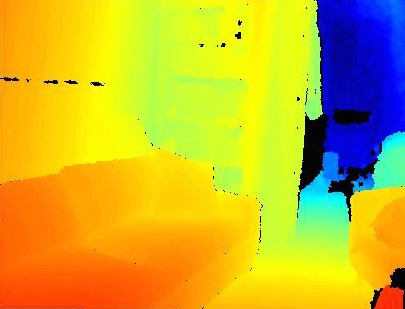
\includegraphics[height=2.1cm]{ogm_ex3.jpeg}\hspace*{0.1cm}
\hspace*{0.5cm}
    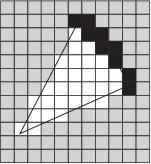
\includegraphics[height=2.1cm]{ogm_ex1.jpg}\hspace*{0.1cm}
\hspace*{0.5cm}
    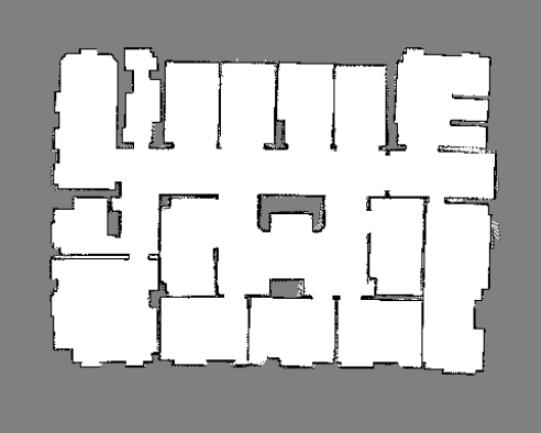
\includegraphics[height=2.1cm]{ogm_ex2.png}\hspace*{0.1cm}
}
\end{figure}}

\end{frame}


\begin{frame}
\frametitle{Problem Definition}

\begin{itemize}
	\item The Map and the Robot
	\begin{itemize}
	\item Map $m$ is composed of $n_m$ grid cells with known location and size
	\item The $i$-th grid cell $\mathbf{m}_i$ is a \emph{static binary} random variable, independent of other grid cells: $P(m)=P(\mathbf{m}_1,\mathbf{m}_2,\ldots,\mathbf{m}_{n_m})=\prod_{i=1}^{n_m}P(\mathbf{m}_i)$
	\item \emph{Pose $X_t$} is known, containing robot \emph{position} and \emph{attitude}
	\end{itemize}
\vspace*{0.0cm}\pause
\end{itemize}
\begin{minipage}[t]{7.0cm}
\begin{itemize}
	\item Depth Measurements
	\begin{itemize}
	\item Each measurement origin and direction is known \emph{deterministically}
	\item A measurement \emph{scan} $Z_t=\braces{z_{t,1},z_{t,2},\ldots,z_{t,n_z}}$ contains $n_z$ measurement \emph{rays} (depths)% at the $t$-th time step, and the history of measurement scans $Z_{1:t}$ is known
\item The \emph{forward sensor model} is known from the sensor properties
\end{itemize}
\end{itemize}
\end{minipage}
\begin{minipage}[t]{3.0cm}
%The \emph{forward sensor model} is the probability density distribution $p(z_{t,l}|m,X_{t})$  known from the sensor properties
\hspace*{0.25cm}
\begin{figure}[!htbp]
\vspace*{-0.25cm}
%\vspace*{0.25cm}
\centerline{
    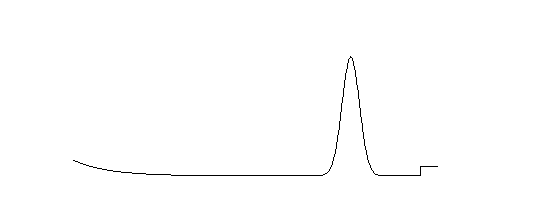
\includegraphics[width=3.5cm]{BeamModel.png}\hspace*{0.1cm}
    }
\vspace*{0.25cm}
\centerline{
    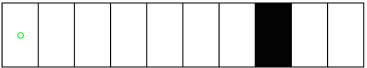
\includegraphics[width=2.5cm]{1D_True_Grid.png}\hspace*{0.1cm}
%    \hspace*{0.75cm}
    }
{Beam Model for Range Finders}
\end{figure}

\end{minipage}



\end{frame}

\begin{frame}
\frametitle{Problem Definition}

\begin{itemize}
	\item Bayesian Framework
	\begin{itemize}
	\item Markov Assumption: latest a priori cell occupancy probabilities capture the information from all prior observations
	\item Log-Odds Ratio: popular representation due to simple additive update structure and probability truncation avoidance, but requires the \emph{assumption}
	\begin{align*}
		P(Z_t|\mathbf{m}_i,X_{1:t},Z_{1:t-1})\approx P(Z_t|\mathbf{m}_i,X_t)
	\end{align*}
	\end{itemize}
\vspace*{0.0cm}\pause
	\item Inverse Sensor Model
	\begin{align*}
P(\mathbf{m}_i|z_{t,l},&X_{1:t},Z_{1:t-1})\nonumber
\\
&=\eta_{t,l} \textcolor{blue}{\sum_{m\in\mathcal{M}_i}}p(z_{t,l}|m,X_{t})P(m|X_{1:t-1},Z_{1:t-1}).
\end{align*}
	\begin{itemize}
	\item Given $n$ grid cells: $\textcolor{blue}{\mathcal O(2^n)}$ is \emph{computationally intractable}, motivating a different solution
	\end{itemize}
\end{itemize}

\end{frame}

\begin{frame}
\frametitle{Related Work }

\begin{minipage}[t]{7.0cm}
\begin{itemize}
	\item Approximate a function for the inverse sensor model based on intuition
	\begin{itemize}
		\item Simple to implement, but mathematically inaccurate
	\end{itemize}
\end{itemize}
\end{minipage}
\begin{minipage}[t]{3.0cm}
\begin{figure}[!htbp]
\centerline{
    \vspace*{-0.5cm}
%	\hspace*{0.25cm}
    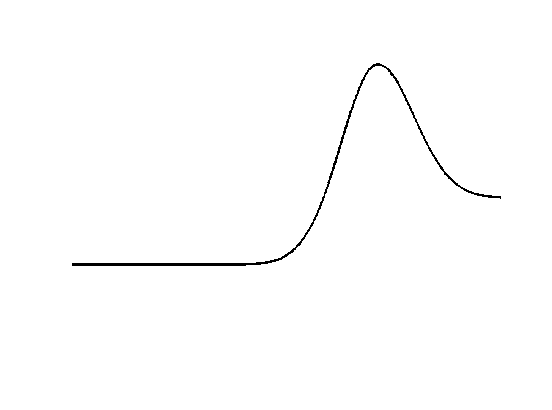
\includegraphics[width=4.0cm]{Approx_ISM_shortened.png}\hspace*{0.1cm}
    }
\centerline{
    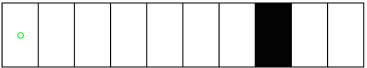
\includegraphics[width=3.5cm]{1D_True_Grid.png}
%    \hspace*{0.75cm}
    }
		\end{figure}
\end{minipage}
\vspace*{-0.5cm}
\begin{itemize}
	\item Find a solution through learning
	\begin{itemize}
		\item Simulate maps, poses, and measurements and use learning to obtain an inverse sensor model
		\item Complicated, unclear how these parameters are chosen
	\end{itemize}
	\item Goal: design a \emph{simple} and \emph{accurate} occupancy grid mapping method avoiding log-odds ratio assumptions
\end{itemize}


\end{frame}



\begin{frame}
\frametitle{Single Measurement Ray}

\begin{itemize}
    \item Main idea: make use of occupancy grid mapping \emph{assumptions} and extract \emph{patterns} from probabilistic properties to find a \emph{computationally-efficient} solution
	\begin{itemize}
		\item Since the origin and direction of each measurement ray is known deterministically, the set of grid cells that the ray intersects is \emph{known through geometry}
		\item A depth reading follows the forward sensor model, which \emph{only depends} on the first occupied grid cell along the measurement ray
	\end{itemize}
\end{itemize}

\begin{figure}[!htbp]
\vspace*{-0.25cm}
\centerline{
	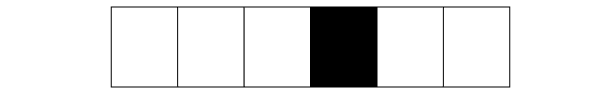
\includegraphics[width=4.0cm]{rkplus_1.png}\hspace*{-0.5cm}
	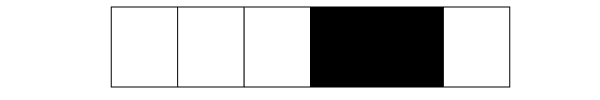
\includegraphics[width=4.0cm]{rkplus_2.png}}
 \centerline{
	
\includegraphics[width=4.0cm]{rkplus_3.png}\hspace*{-0.5cm}
	
\includegraphics[width=4.0cm]{rkplus_4.png}}
\end{figure}

\end{frame}




\begin{frame}
\frametitle{Single Measurement Ray}
\begin{itemize}
    \item Reduced Map
	\begin{itemize}
		\item Consider a reduced map of the $l$-th measurement ray, namely $r_l=\braces{\mathbf{r}_{l,1},\mathbf{r}_{l,2},\ldots,\mathbf{r}_{l,n_{r,l}}}$, consisting of grid cells \emph{intersected} by the measurement ray within the sensor limits, \emph{indexed by increasing distance}
		\item Since reduced map $r_l$ is composed of binary random variables, it has \emph{$2^{n_{r,l}}$} possible solutions
		\item However, the combinations of possible maps are grouped based on the \emph{closest occupied cells}
		\item Probability calculations have several repeated terms, and may be determined \emph{recursively}
		\item The number of possible map combinations is just \emph{$n_{r,l}+1$}
%		\item If $\mathbf{r}_{l,1}$ is occupied (a priori probability $P(\mathbf{r}_{l,1}|X_{1:t-1},Z_{1:t-1})$), then each occupancy $\mathbf{r}_{l,2:n_{r,l}}$ does \emph{not} affect forward sensor model $P(z_{t,l}|\mathbf{r}_{l,1},X_t)$
%		\item Similarly, if $\mathbf{r}_{l,2}$ is occupied (a priori probability $P(\bar{\mathbf{r}}_{l,1}|X_{1:t-1},Z_{1:t-1})P(\mathbf{r}_{l,2}|X_{1:t-1},Z_{1:t-1})$), then forward sensor model $P(z_{t,l}|\mathbf{r}_{l,2},X_t)$ is independent of grid cells of higher index
%		\item This concept is extended for all grid cells in $r_l$
	\end{itemize}
\end{itemize}
\end{frame}

%\begin{frame}
%\frametitle{Single Measurement Ray}
%\begin{itemize}
%	\item Let $P(\mathbf{r}_{l,k}|z_{t,l},X_{1:t},Z_{1:t-1})=\eta_{t,l}\tilde P(\mathbf{r}_{l,k}|z_{t,l},X_{1:t},Z_{1:t-1})$
%	\item The $k$-th unnormalized probability is written generally as
%	{\tiny
%	\begin{align*}
%		& \tilde P(\mathbf{r}_{l,k}|z_{t,l},X_{1:t},Z_{1:t-1})\\\nonumber&\quad=P(\mathbf{r}_{l,k}|X_{1:t-1},Z_{1:t-1})\nonumber\\&\quad\qquad\times 
%		\bigg[\sum_{i=1}^{k-1}\bigg\{\prod_{j=0}^{i-1}P(\bar{\mathbf{r}}_{l,j}|X_{1:t-1},Z_{1:t-1})\bigg\}p(z_{t,l}|\mathbf{r}_{l,i+},X_t)P(\mathbf{r}_{l,i}|X_{1:t-1},Z_{1:t-1})\bigg]\nonumber\\
%		&\quad\quad +\qquad\quad \ \ \bigg\{\prod_{j=0}^{k-1}P(\bar{\mathbf{r}}_{l,j}|X_{1:t-1},Z_{1:t-1})\bigg\} p(z_{t,l}|\mathbf{r}_{l,k+},X_t)P(\mathbf{r}_{l,k}|X_{1:t-1},Z_{1:t-1})
%	\end{align*}
%	}
%	\pause
%	\item The \emph{normalizer} $\eta_{t,l}$ is
%	{\tiny
%	\begin{align*}
%		\eta_{t,l}=
%		\bigg[\sum_{i=1}^{n_{r,l}+1}\bigg\{\prod_{j=0}^{i-1}P(\bar{\mathbf{r}}_{l,j}|X_{1:t-1},Z_{1:t-1})\bigg\}p(z_{t,l}|\mathbf{r}_{l,i+},X_t)P(\mathbf{r}_{l,i}|X_{1:t-1},Z_{1:t-1})\bigg]^{-1}
%	\end{align*}
%	}
%\end{itemize}
%\end{frame}


\begin{frame}
\frametitle{Practical Implications}

\begin{itemize}
	\item Computational Efficiency
	\begin{itemize}
%		\item Several of the terms required for $\eta_{t,l}$ and $\tilde P(\mathbf{r}_{l,k}|z_{t,l},X_{1:t},Z_{1:t-1})$ for each $k=1,2,\ldots,n_{r,l}$ are repeated and need not be computed more than once
		\item \emph{Computational order $\mathcal O(n_{r,l}+1)$} for all grid cells in reduced map $r$: each grid cell once and the empty map case
		\item It is commonly believed that the computational order is $\mathcal O(2^{n_{r,l}})$; the proposed method is \emph{$2^{n_{r,l}}\left(\frac{n_{r,l}}{n_{r,l}+1}\right)$ times faster} for the \emph{same solution}
		\item Proposed method completely avoids inaccuracies associated with heuristic solutions, learned methods, and log-odds ratio update assumptions
%		\item Analytic solution is valid for any forward sensor model dependent on the closest occupied space
	\end{itemize}
	\item A \emph{ray-by-ray} approach accounts for all measurements rays composing a measurement \emph{scan}
		\begin{align*}
			P(m|X_{1:t}&,Z_{1:t})=P((\dots(((m|X_{1:t},Z_{1:t-1})|z_{t,1})|z_{t,2})|\ldots)|z_{t,n_z})
		\end{align*}
\end{itemize}
\end{frame}




\begin{frame}
\frametitle{Numerical Example}

\begin{minipage}[t]{5.0cm}
\vspace*{0.5cm}
\begin{itemize}
	\item A standard \emph{approximate} inverse sensor model technique is compared with the proposed \emph{exact} method
\end{itemize}
\end{minipage}
\begin{minipage}[t]{5.0cm}
%\vspace*{0.5cm}
\begin{figure}[!htbp]
    \centering
    \begin{subfigure}{0.5\textwidth}
        \centering
        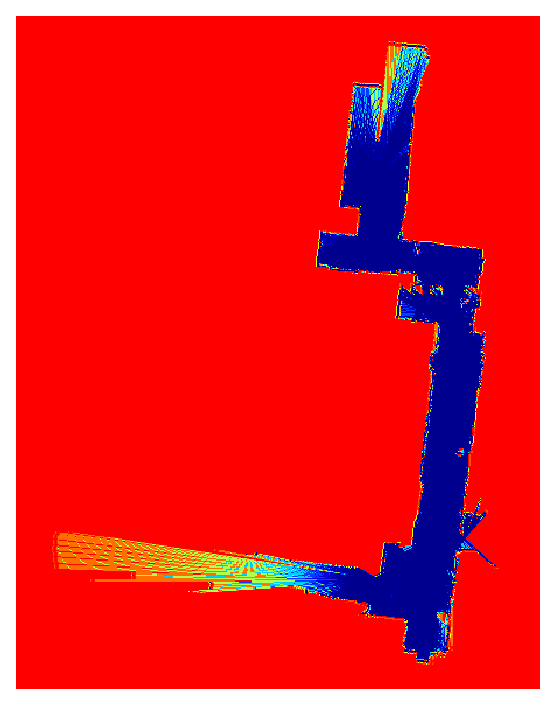
\includegraphics[width=\textwidth]{AISM_Image_inf_19.pdf}
        \caption*{Approximate}
    \end{subfigure}
    \hspace*{-0.1\textwidth}
    \begin{subfigure}{0.5\textwidth}
        \centering
        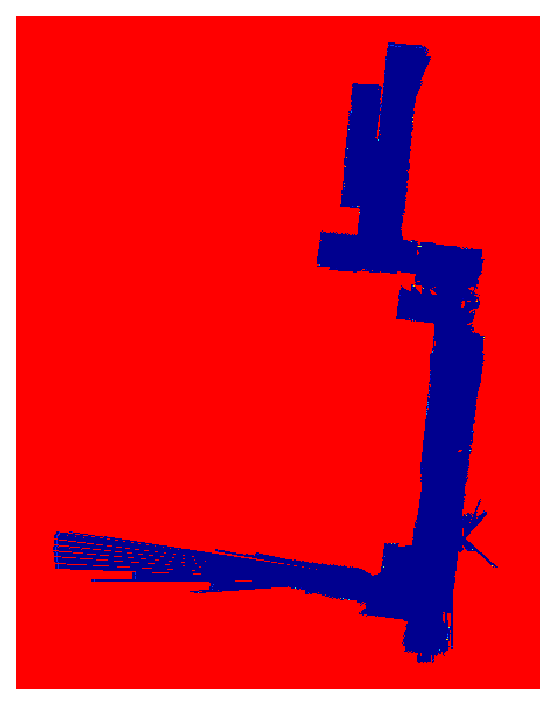
\includegraphics[width=\textwidth]{EISM_Image_inf_19.pdf}
        \caption*{Exact}
    \end{subfigure}
\end{figure}
\end{minipage}

%\begin{figure}[!ht]
%    \centering
%    \begin{subfigure}[t]{0.35\columnwidth}
%        \centering
%        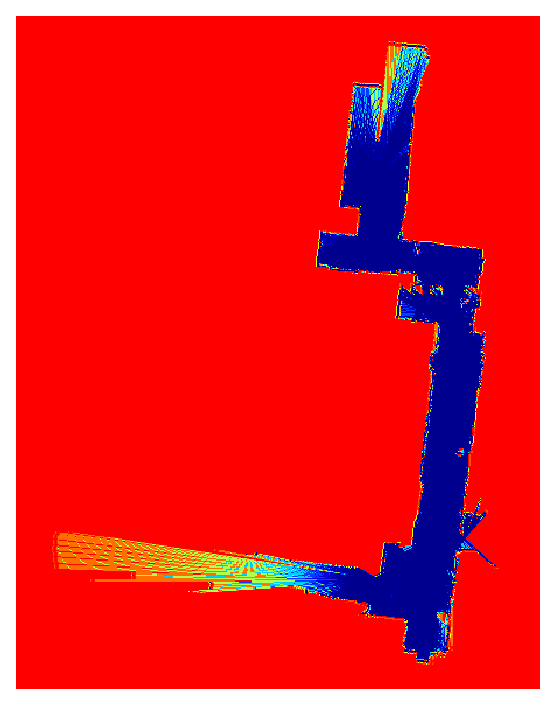
\includegraphics[width=0.5\textwidth]{AISM_Image_inf_19.pdf}
%        \caption*{Approximate}
%    \end{subfigure}
%    \hspace*{0.5cm}
%    \begin{subfigure}[t]{0.35\columnwidth}
%        \centering
%        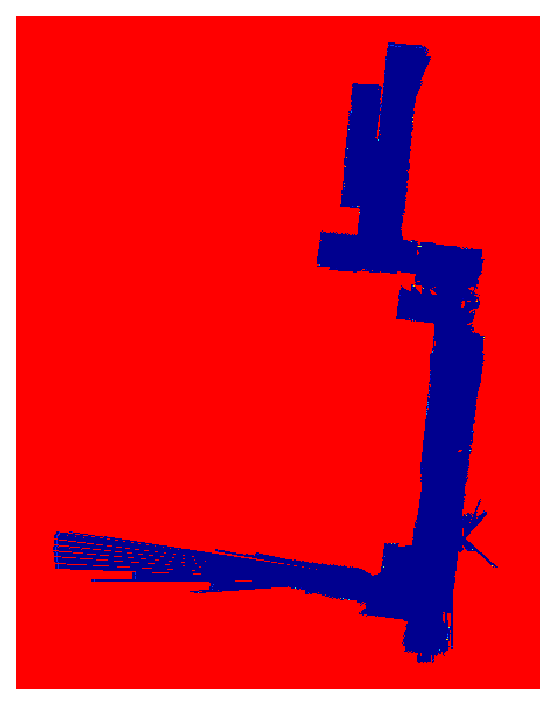
\includegraphics[width=0.5\textwidth]{EISM_Image_inf_19.pdf}
%        \caption*{Exact}
%    \end{subfigure}
%\end{figure}

\begin{itemize}
\item The exact algorithm yields a more \emph{certain} map from the same measurement set
\end{itemize}

\end{frame}


\section*{}

\begin{frame}
\frametitle{}
%\center
\center{\bf \color{blue} Single-Robot Autonomous Exploration}
\end{frame}


\subsection*{Single-Robot Autonomous Exploration}

\begin{frame}
\frametitle{Introduction}
\begin{itemize}
        	\item The environment is initially uncertain, so the robot path is initially unknown
	\item Simultaneous localization and mapping assumes robotic actions are provided
	\item Human interaction is common to guide the robot
	\item Goal: develop effective policies to govern robotic motion 
\end{itemize}

\end{frame}


\begin{frame}
\frametitle{Problem Definition}
\begin{itemize}
        	\item Uncertainty-Based Exploration
	\begin{itemize}
		\item Main idea: choose robot motions that minimize the uncertainty of the occupancy grid map
		\item Equivalently maximize map information gain
	\end{itemize}
\end{itemize}
\begin{minipage}[t]{7.0cm}
\begin{itemize}
	\item Entropy
	\begin{itemize}		
		\item \emph{Shannon's entropy} serves as an uncertainty measure
		\begin{align*}
			H(P)=-P\log P-\bar{P}\log \bar{P}%-(1-P)\log(1-P)
		\end{align*}
		with cell occupancy probability $P$ and complement $\bar{P}=1-P$
		\item Entropy $H$ is maximized when $P=0.5$ and minimized as $P\rightarrow0$ or $P\rightarrow1$
	\end{itemize}
\end{itemize}
\end{minipage}
\begin{minipage}[t]{3.0cm}
\vspace*{0.5cm}
\begin{figure}[!htbp]
	\centerline{
		\hspace*{1.25cm}
   		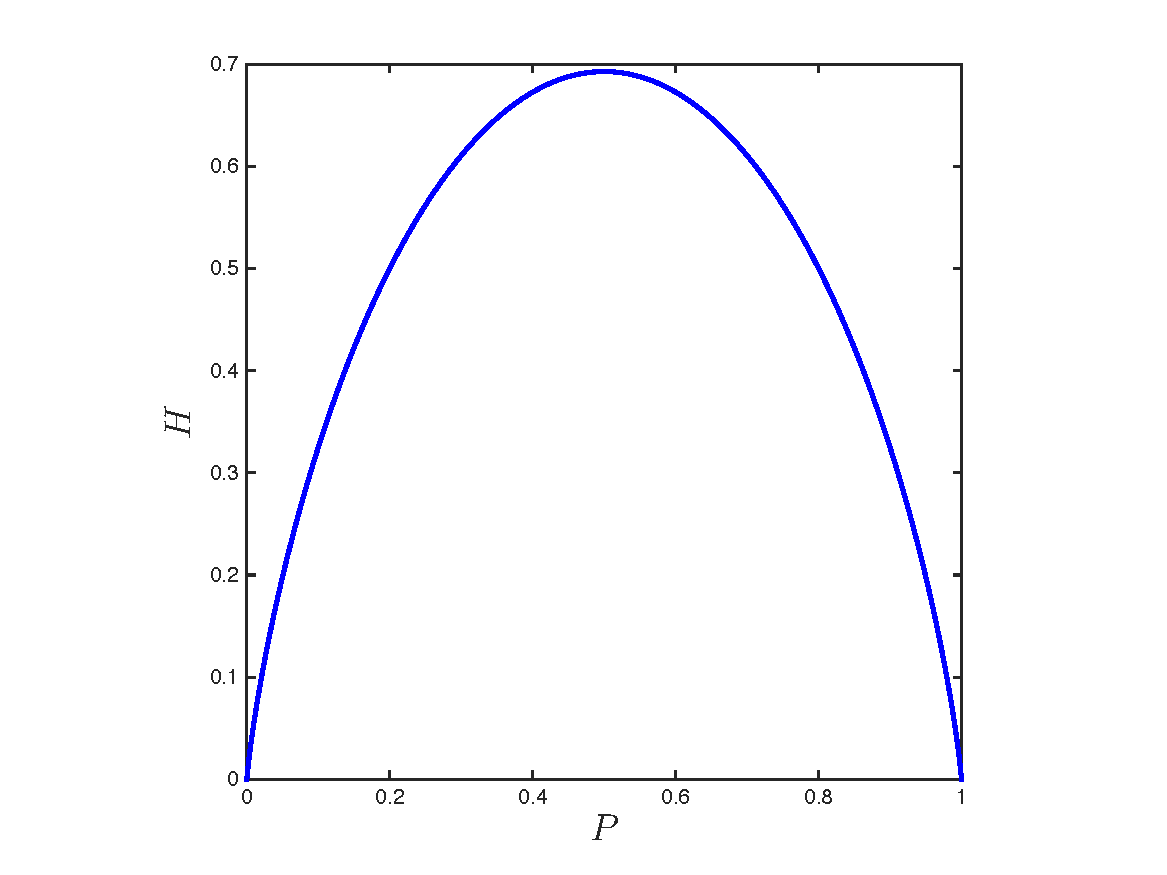
\includegraphics[width=5.0cm]{H_Plotted_square.pdf}%\hspace*{0.1cm}
	}
\end{figure}
\end{minipage}

\end{frame}



\begin{frame}
\frametitle{Problem Definition}
\begin{itemize}
        	\item Map Information Gain Maximization
	\begin{itemize}
		\item Goal: choose a set of optimal future poses to maximize map information gain
		\pause
		\item Challenge: the complete set cannot be calculated accurately with an initially highly-uncertain environment
		\pause
		\item Solution: choose short-term optimal pose goals, reevaluating an updated map for the subsequent optimizations
		\pause
		\item The information gain considering candidate future pose $X_c$:% is
		\begin{align*}
			\mathcal I(X_c)&=H(P(m|X_{1:t},Z_{1:t}))-\text{E}\left[H(P(m|X_{1:t},Z_{1:t},X_c,Z_c))\right]
		\end{align*}
		\pause
		\item Optimal pose $X^*_c$ satisfies
		\begin{align*}
			X_c^*=\argmax_{X_c}{\mathcal I(X_c)}
		\end{align*}
	\end{itemize}
\end{itemize}


\end{frame}



\begin{frame}
\frametitle{Related Work}
\begin{itemize}
        	\item Frontier-Based Exploration
	\begin{itemize}
		\item Main idea: robot moves toward boundaries between certain and uncertain space, takes measurements, then pushes back the boundaries
		\item Non-entropy-based exploration
		\item Heuristic
	\end{itemize}
	\pause
	\item Entropy-Based Exploration
	\begin{itemize}
		\item Cell occupancy probabilities are inaccurate: inverse sensor model is heuristic or learned, and frequently estimated with Rao-Blackwellized particle filters
		\item Inaccurate probabilities imply inaccurate entropy measures
		\item Approaches use ``hallucination measurements'' to predict how future measurements \emph{might} affect the map uncertainty,
		\begin{align*}
			\text{E}\left[H(P(m|X_{1:t},Z_{1:t},X_c,Z_c))\right]\approx H(P(m|X_{1:t},Z_{1:t},X_c,\text{E}\left[Z_c\right]))
		\end{align*}
	\end{itemize}
\end{itemize}


\end{frame}


\begin{frame}
\frametitle{Direct Entropy Calculation}
\begin{itemize}
        	\item Instead of relying on frontiers or making assumptions about measurements, the expected map entropy is \emph{calculated directly} by the law of total expectation:
	\begin{align*}
		\text{E}[H(P(m|X,z))]=\int_{z_\text{min}}^{z_\text{max}}
		H(P(m|X,z))p(z|X)dz,
	\end{align*}
	\item The robot pose is chosen to maximize map information gain from this expectation
	\item Dijkstra's algorithm provides collision-free waypoints for the robot path
	\item Smooth trajectory: constrained polynomial least squares 
\end{itemize}


\end{frame}


\begin{frame}
\frametitle{Numerical Example}
\begin{itemize}
        	\item A benchmark example floor plan is explored and mapped using the proposed mapping and exploration algorithms
	\item Simulations in Robot Operating System (ROS)
\end{itemize}
\begin{figure}
    \centering
    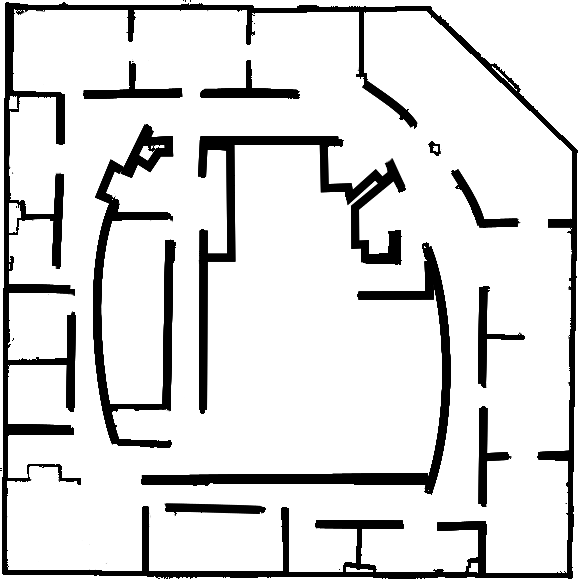
\includegraphics[width=0.4\textwidth]{intel_clean.png}
    \caption*{Modified Intel Research Lab floor plan form the SLAM benchmark}
\end{figure}

\end{frame}

%\begin{frame}
%\frametitle{Numerical Results}
%	\centering{
%	\includemovie[poster,autoplay]{0.720\textwidth}{0.576\textwidth}{JIRS16_simulation_speedup10x_then_speedup100x.mov}}
%\end{frame}

\begin{frame}
\frametitle{Numerical Results}

\begin{figure}[!ht]
    \centering
    \begin{subfigure}[t]{0.2\columnwidth}
        \centering
        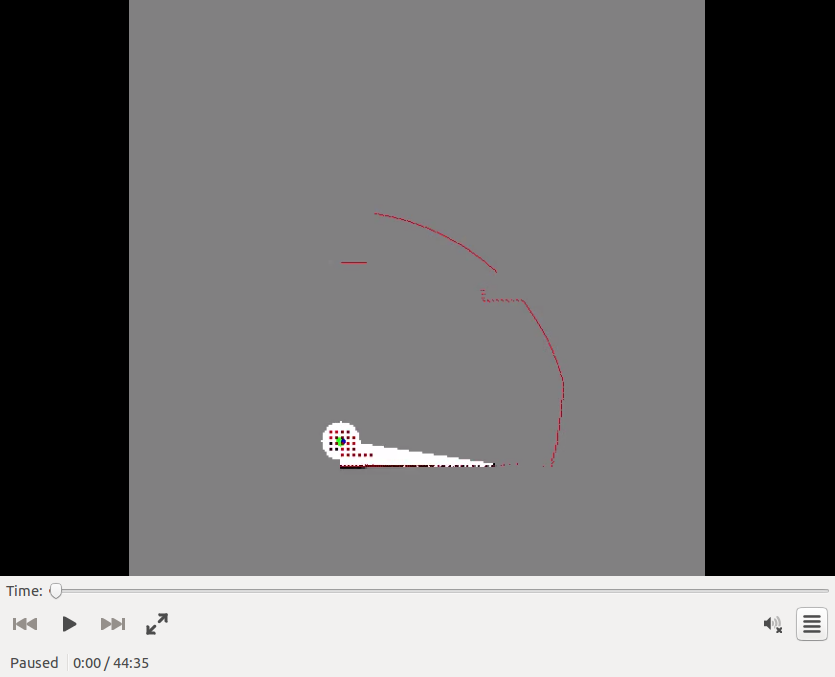
\includegraphics[trim = {4.6cm 3.8cm 4.6cm 0}, clip, width=\textwidth]{0min.png}
        \caption*{$t=0$ min}
        \label{fig:IRL0min}
    \end{subfigure}
    \begin{subfigure}[t]{0.2\columnwidth}
        \centering
        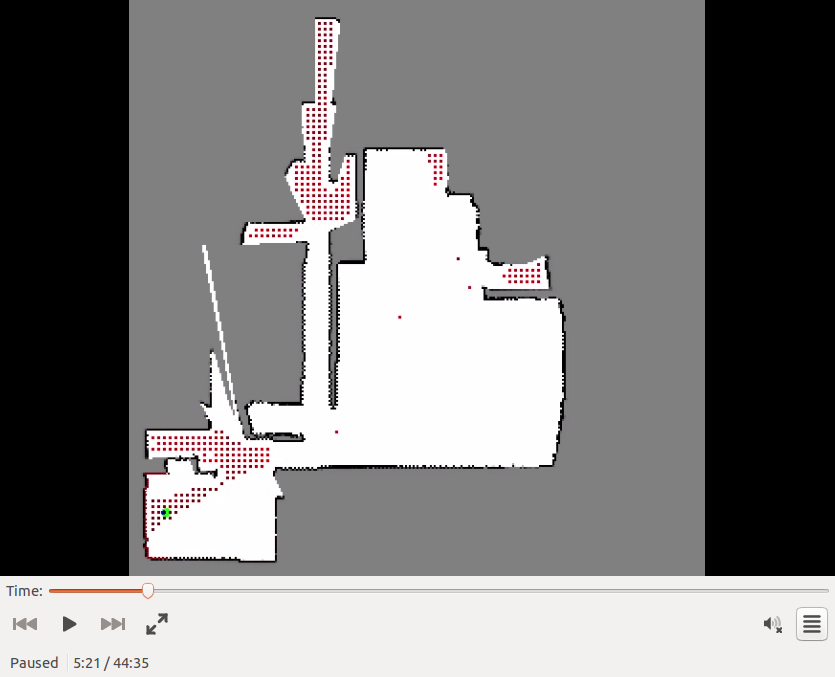
\includegraphics[trim = {4.6cm 3.8cm 4.6cm 0}, clip, width=\textwidth]{5min.png}
        \caption*{$t=5$ min}
        \label{fig:IRL5min}
    \end{subfigure}
    \begin{subfigure}[t]{0.2\columnwidth}
           \centering
           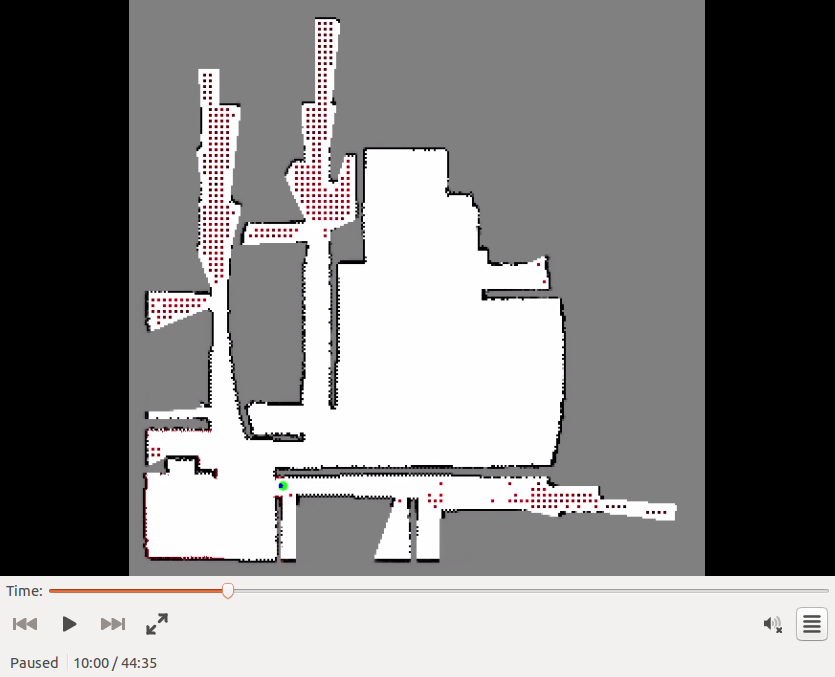
\includegraphics[trim = {4.6cm 3.8cm 4.6cm 0}, clip, width=\textwidth]{10min.png}
        \caption*{$t=10$ min}
        \label{fig:IRL10min}
    \end{subfigure}
    \begin{subfigure}[t]{0.2\columnwidth}
           \centering
           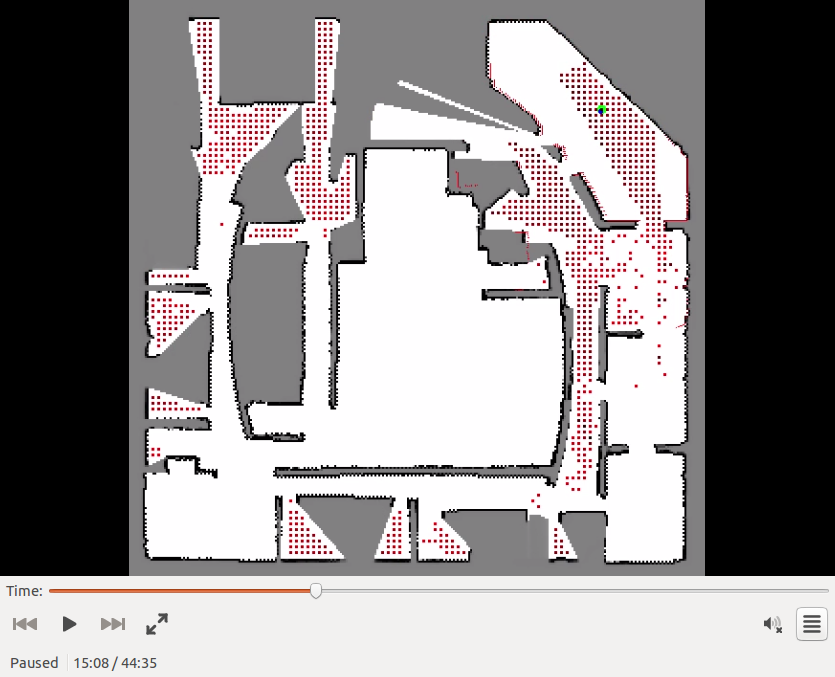
\includegraphics[trim = {4.6cm 3.8cm 4.6cm 0}, clip, width=\textwidth]{15min.png}
        \caption*{$t=15$ min}
        \label{fig:IRL15min}
    \end{subfigure}
    \begin{subfigure}[t]{0.2\columnwidth}
         \centering
         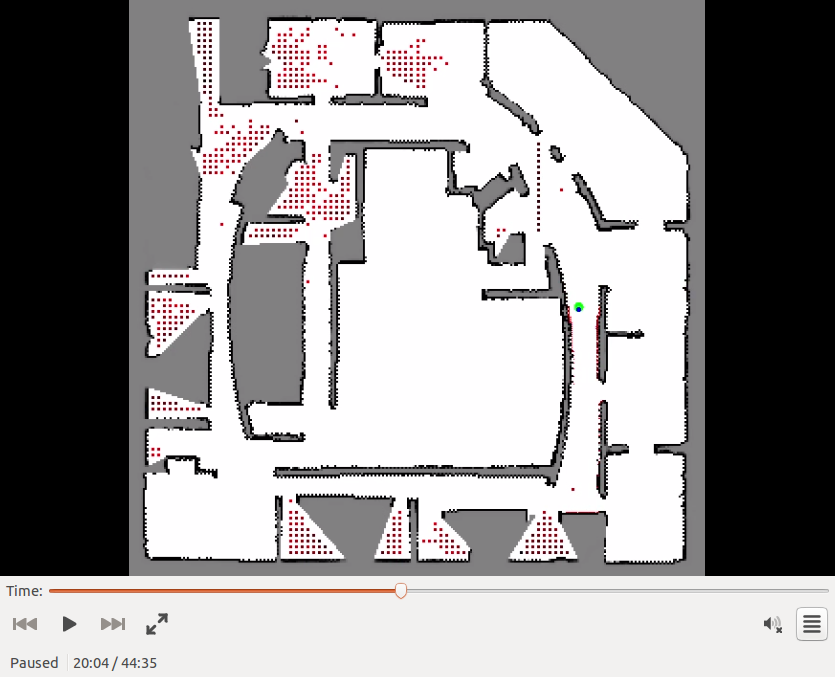
\includegraphics[trim = {4.6cm 3.8cm 4.6cm 0}, clip, width=\textwidth]{20min.png}
        \caption*{$t=20$ min}
        \label{fig:IRL20min}
    \end{subfigure}
    \begin{subfigure}[t]{0.2\columnwidth}
           \centering
           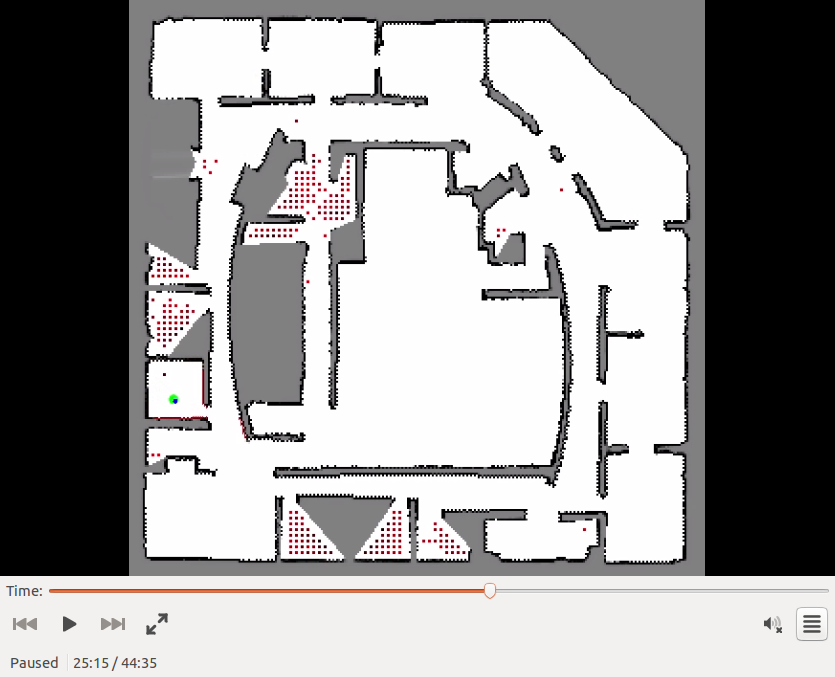
\includegraphics[trim = {4.6cm 3.8cm 4.6cm 0}, clip, width=\textwidth]{25min.png}
        \caption*{$t=25$ min}
        \label{fig:IRL25min}
    \end{subfigure}
    \begin{subfigure}[t]{0.2\columnwidth}
           \centering
           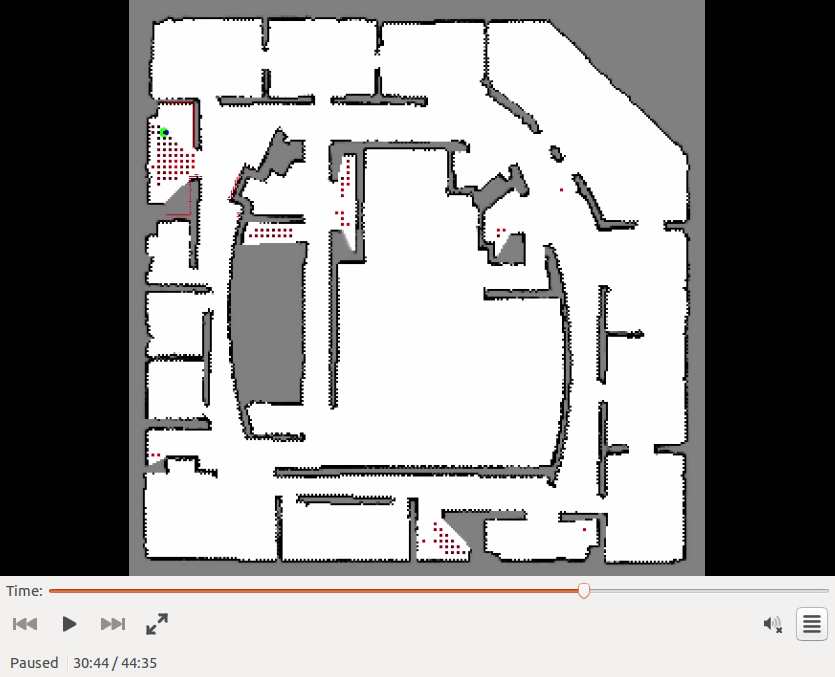
\includegraphics[trim = {4.6cm 3.8cm 4.6cm 0}, clip, width=\textwidth]{30min.png}
        \caption*{$t=30$ min}
        \label{fig:IRL30min}
    \end{subfigure}
    \begin{subfigure}[t]{0.2\columnwidth}
           \centering
           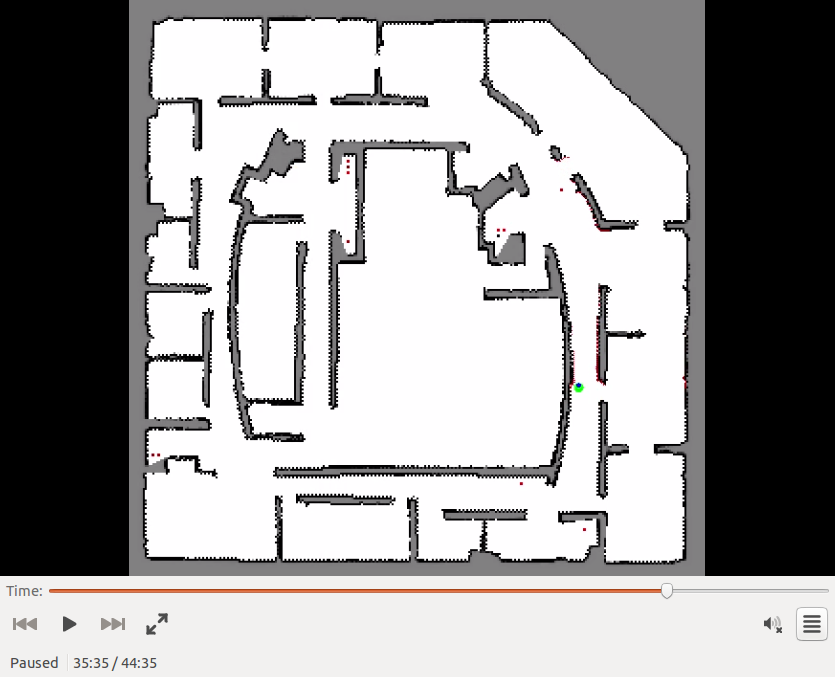
\includegraphics[trim = {4.6cm 3.8cm 4.6cm 0}, clip, width=\textwidth]{35min.png}
        \caption*{$t=35$ min}
        \label{fig:IRL35min}
    \end{subfigure}
%    \begin{subfigure}[t]{0.2\columnwidth}
%           \centering
%           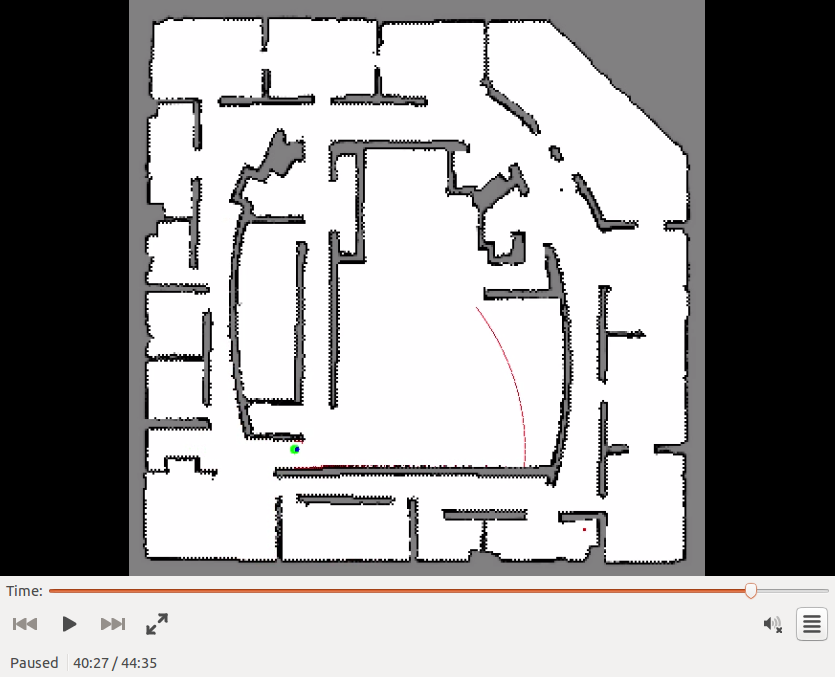
\includegraphics[trim = {4.6cm 3.8cm 4.6cm 0}, clip, width=\textwidth]{40min.png}
%        \caption*{$t=40$ min}
%        \label{fig:IRL40min}
%    \end{subfigure}
    \caption*{A robot (green) measures a room in ROS Stage simulator using modified Intel Research Lab floor plan using the proposed mapping and exploration algorithms.}
    \label{fig:IRL}
\end{figure}


\end{frame}





\begin{frame}
\frametitle{Experimental Example}
\begin{itemize}
        	\item A pioneer ground vehicle explores a room composed of Styrofoam walls
	\item Experiments use ROS, a Microsoft Kinect depth sensor, and Vicon Tracker for pose information
\end{itemize}
\begin{figure}
	\centering
    	\begin{subfigure}[b]{0.28\textwidth}
        		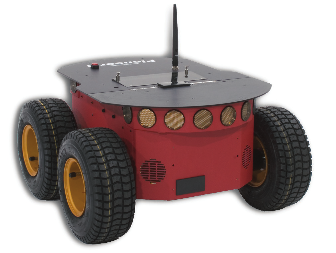
\includegraphics[width=\textwidth]{pioneer.png}
        		\caption*{Pioneer}
    	\end{subfigure}    	
	\hspace*{0.04\textwidth}
	\begin{subfigure}[b]{0.28\textwidth}
        		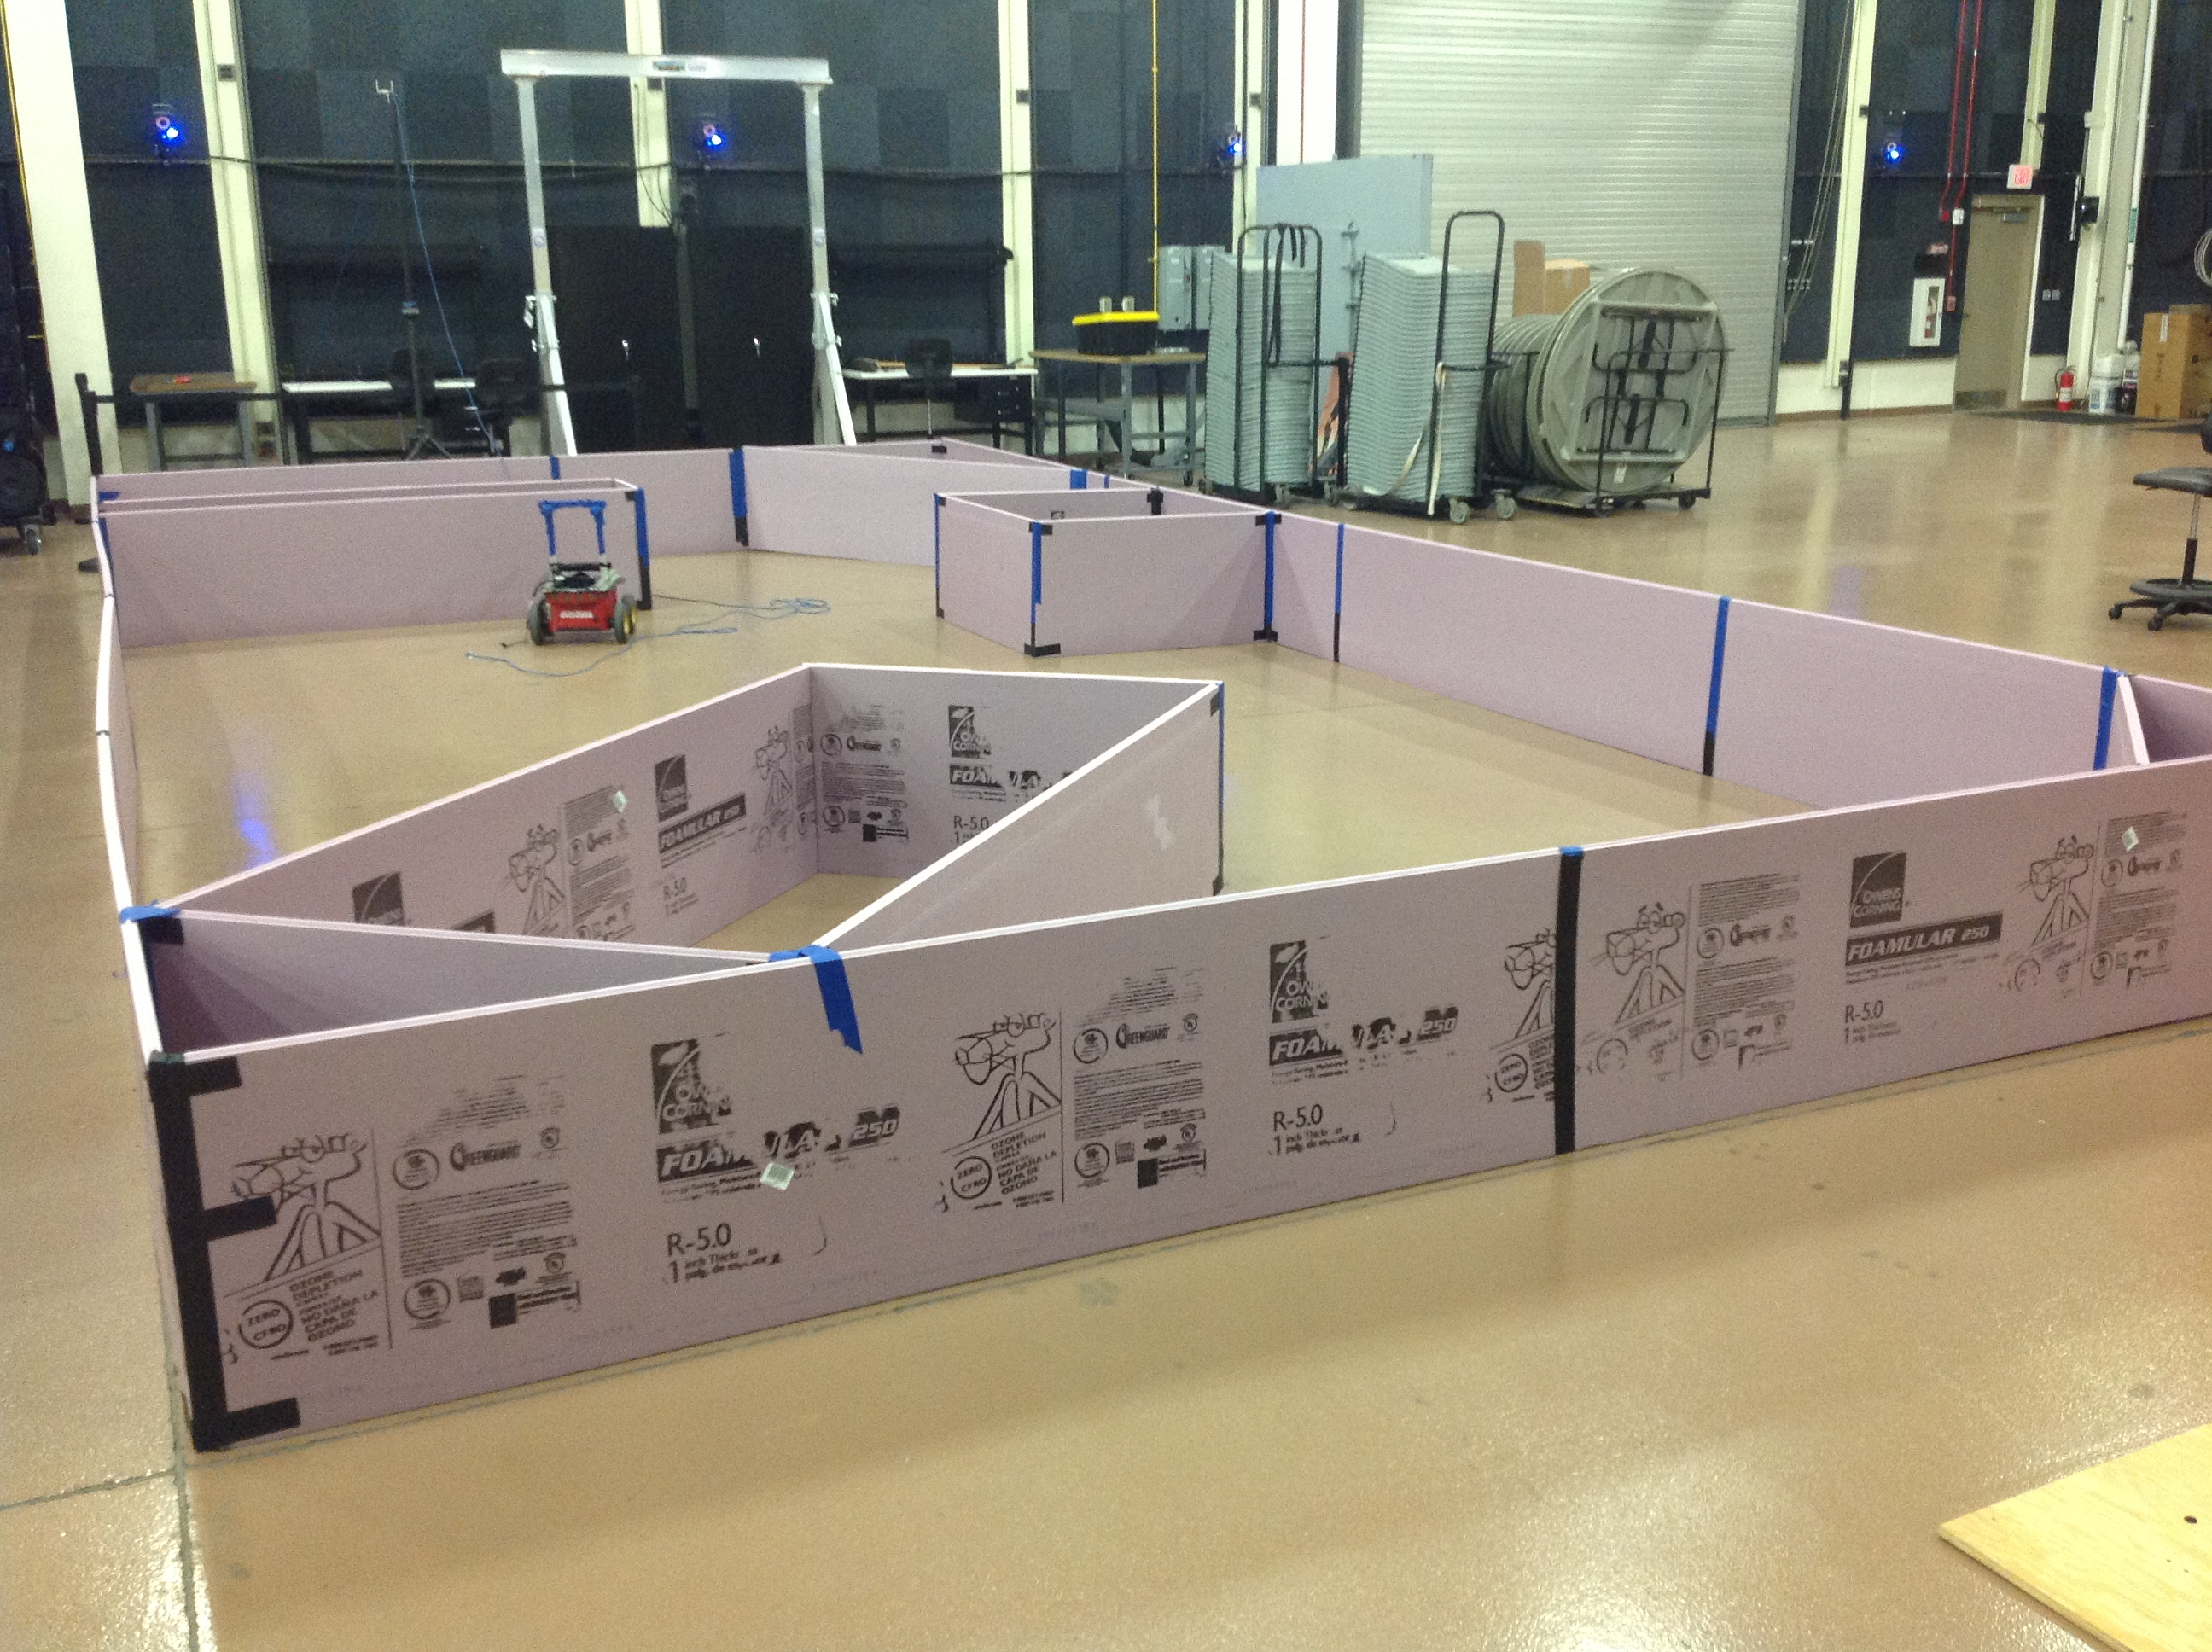
\includegraphics[width=\textwidth]{test_setup_1.jpg}
        		\caption*{Bottom-left view}
    	\end{subfigure}
	\hspace*{0.03\textwidth}
	\begin{subfigure}[b]{0.28\textwidth}
        		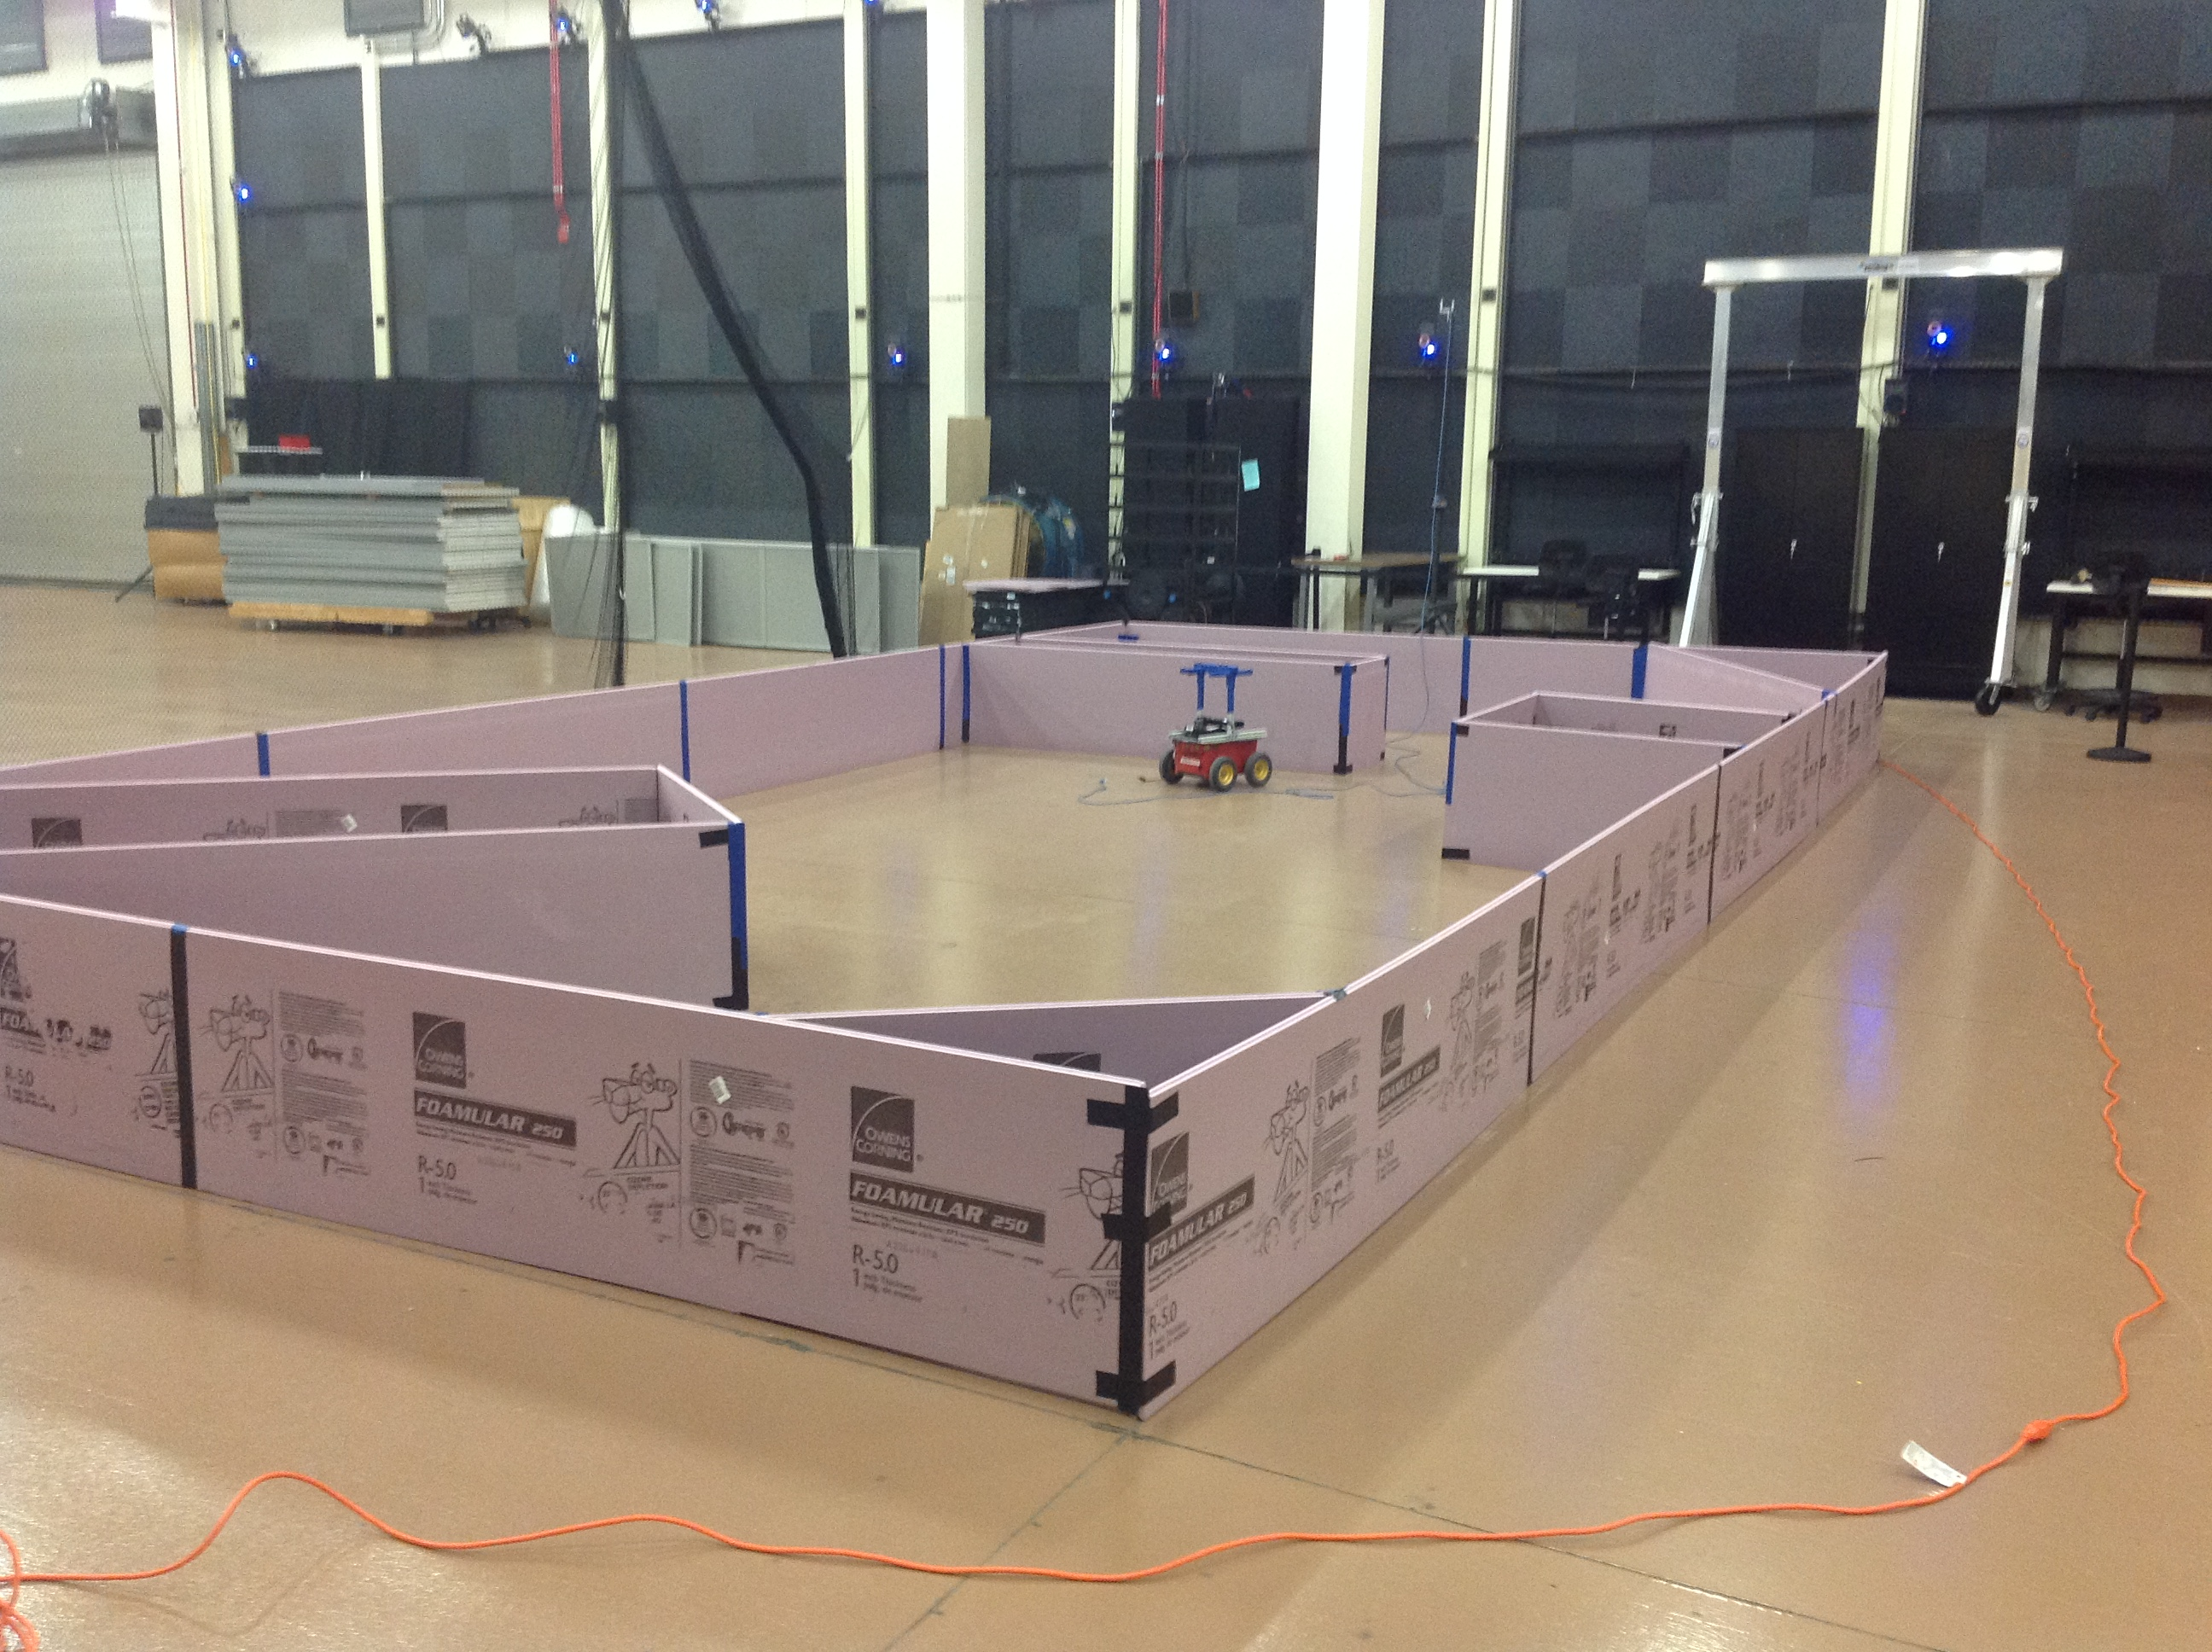
\includegraphics[width=\textwidth]{test_setup_2.jpg}
        		\caption*{Bottom-right view}
    	\end{subfigure}
\end{figure}

\end{frame}

%\begin{frame}
%\frametitle{Experimental Results}
%	\centering{
%	\includemovie[poster,autoplay]{0.720\textwidth}{0.576\textwidth}{JIRS16_experiment_SideBySide_speedup8x.mov}}
%\end{frame}

\begin{frame}
\frametitle{Experimental Results}

\begin{figure}
	\centering{
    	\begin{subfigure}[b]{0.19\textwidth}
        		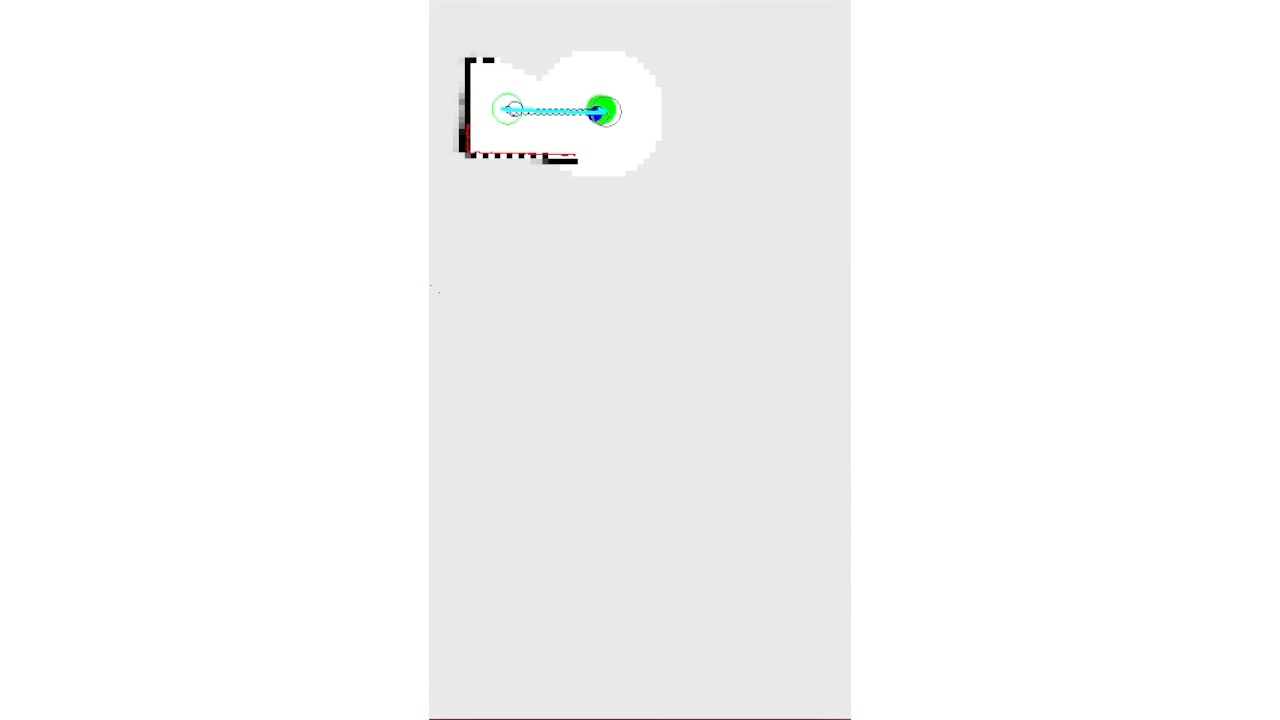
\includegraphics[trim={13cm 1cm 13cm 0}, clip, width=\textwidth]{t_start.jpg}
        		\caption*{$t=0.0$min}
        		\label{fig:Experiment_ogm_t0}
    	\end{subfigure}
	\begin{subfigure}[b]{0.19\textwidth}
        		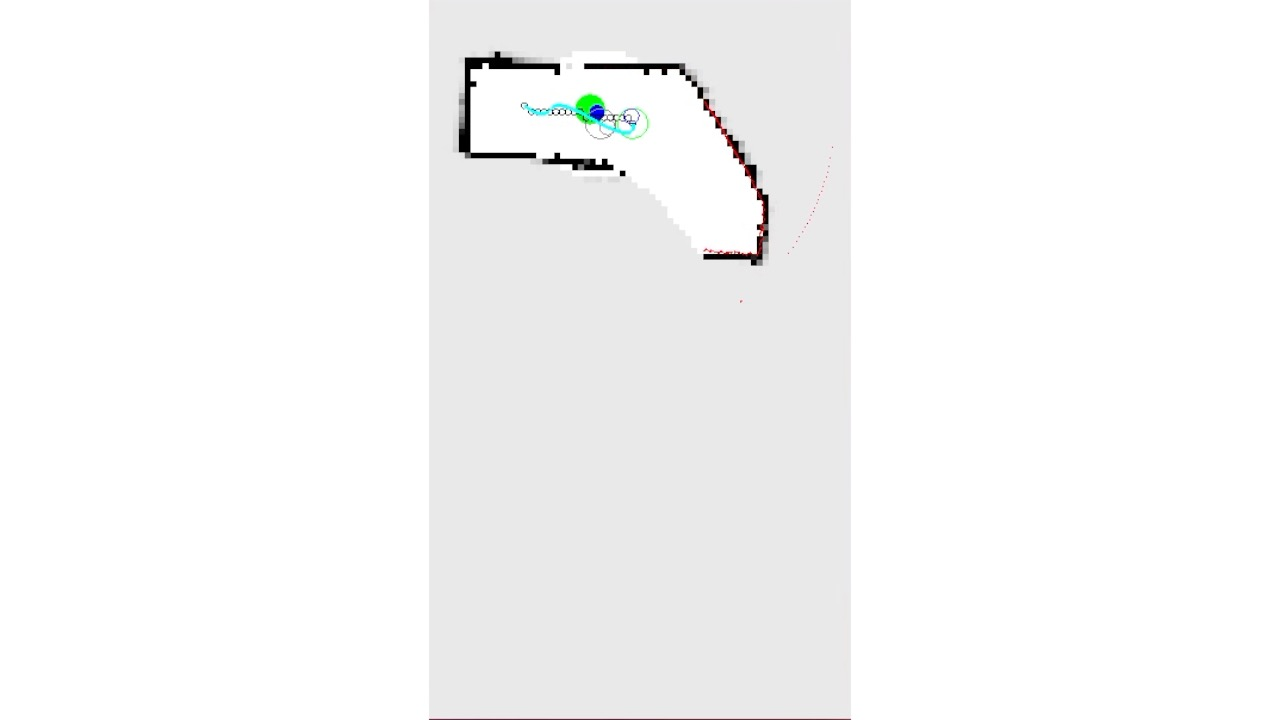
\includegraphics[trim={13cm 1cm 13cm 0}, clip, width=\textwidth]{t_0p5min.jpg}
        		\caption*{$t=0.5$min}
        		\label{fig:Experiment_ogm_t0p5}
    	\end{subfigure}    
	\begin{subfigure}[b]{0.19\textwidth}
        		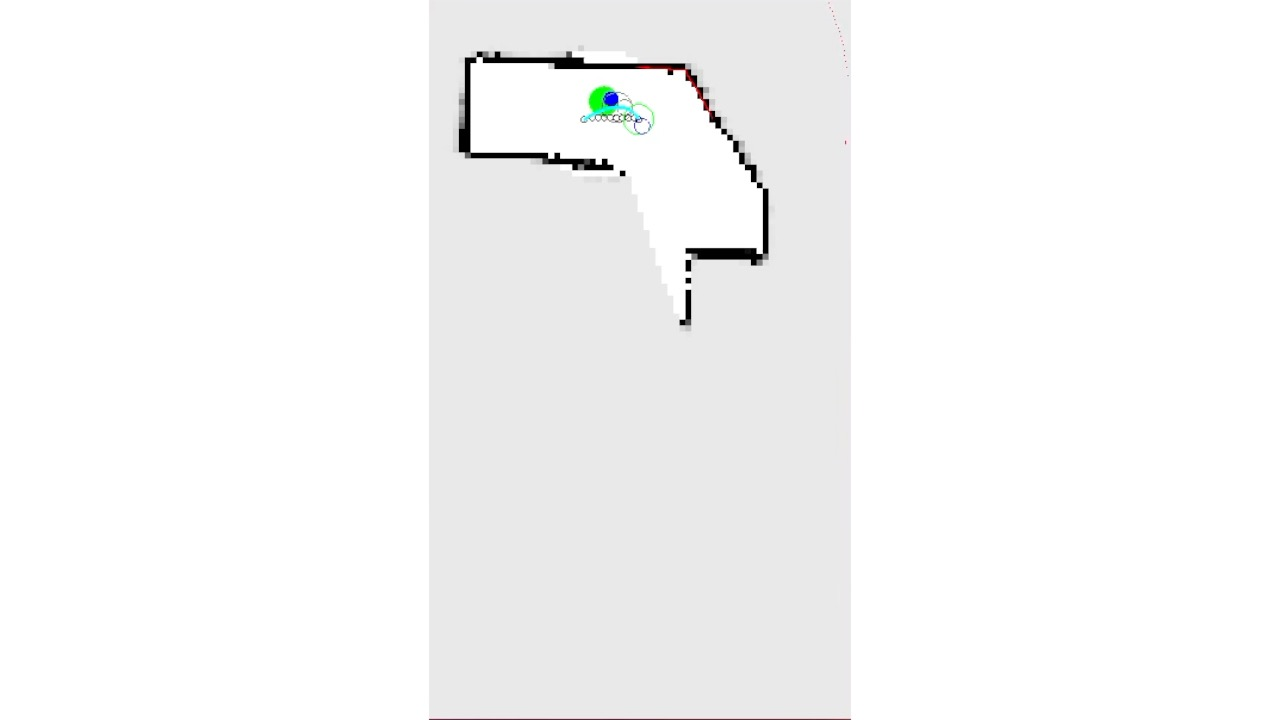
\includegraphics[trim={13cm 1cm 13cm 0}, clip, width=\textwidth]{t_1min.jpg}
        		\caption*{$t=1.0$min}
        		\label{fig:Experiment_ogm_t1}
    	\end{subfigure}
	\begin{subfigure}[b]{0.19\textwidth}
        		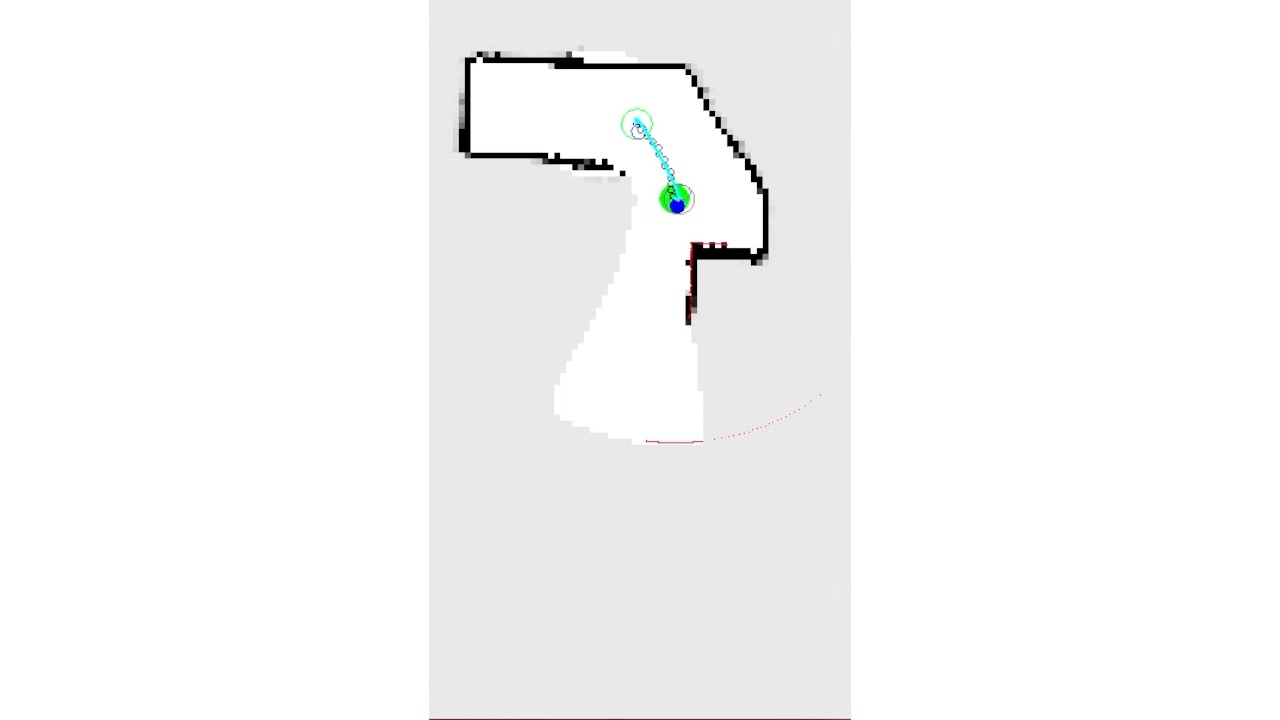
\includegraphics[trim={13cm 1cm 13cm 0}, clip, width=\textwidth]{t_1p5min.jpg}
        		\caption*{$t=1.5$min}
        		\label{fig:Experiment_ogm_t1p5}
    	\end{subfigure}
	\begin{subfigure}[b]{0.19\textwidth}
        		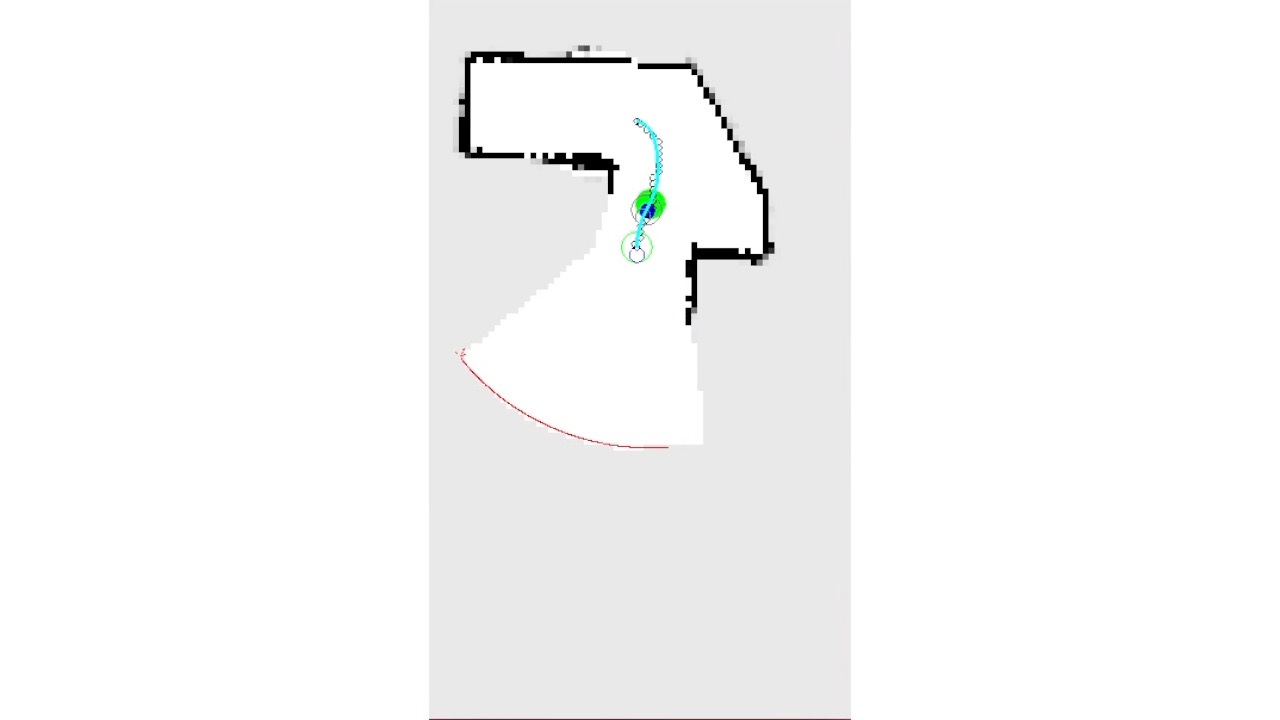
\includegraphics[trim={13cm 1cm 13cm 0}, clip, width=\textwidth]{t_2min.jpg}
        		\caption*{$t=2.0$min}
        		\label{fig:Experiment_ogm_t2}
    	\end{subfigure}
		\vspace*{0.05\textwidth}

	}
	\vspace*{-1cm}
	\centering{
    	\begin{subfigure}[b]{0.19\textwidth}
        		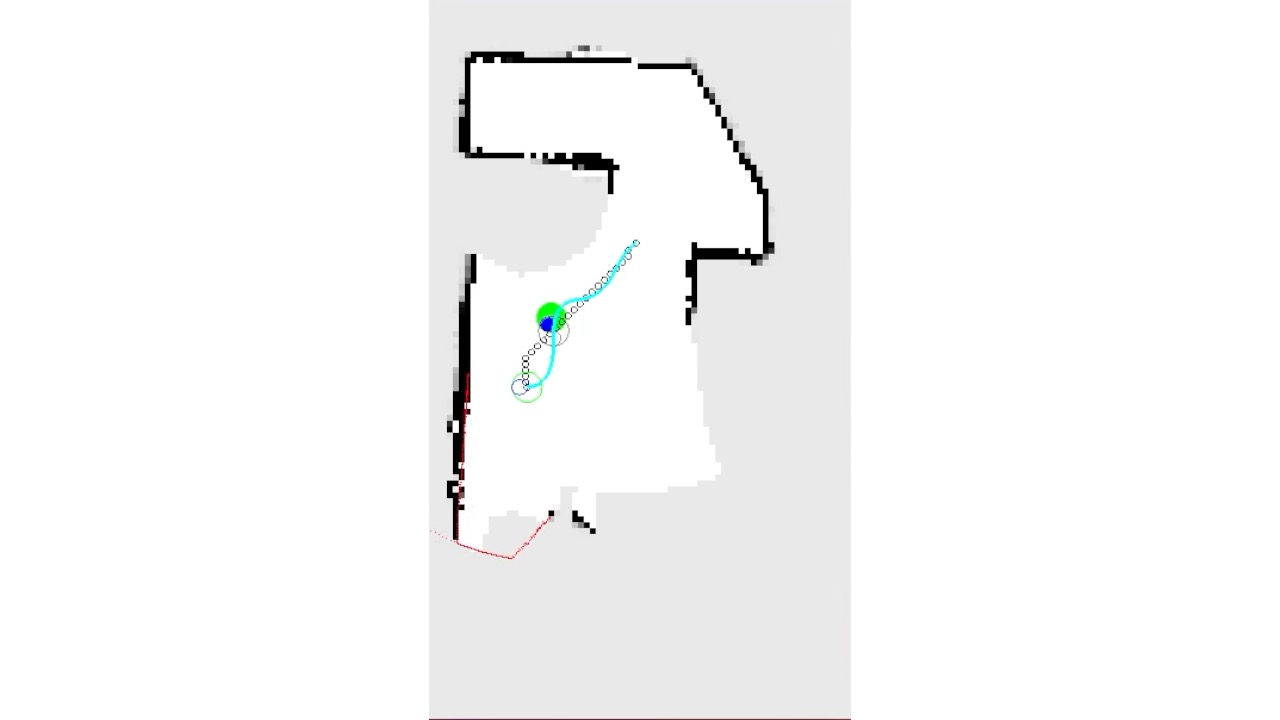
\includegraphics[trim={13cm 1cm 13cm 0}, clip, width=\textwidth]{t_2p5min.jpg}
        		\caption*{$t=2.5$min}
        		\label{fig:Experiment_ogm_t2p5}
    	\end{subfigure}
	\begin{subfigure}[b]{0.19\textwidth}
        		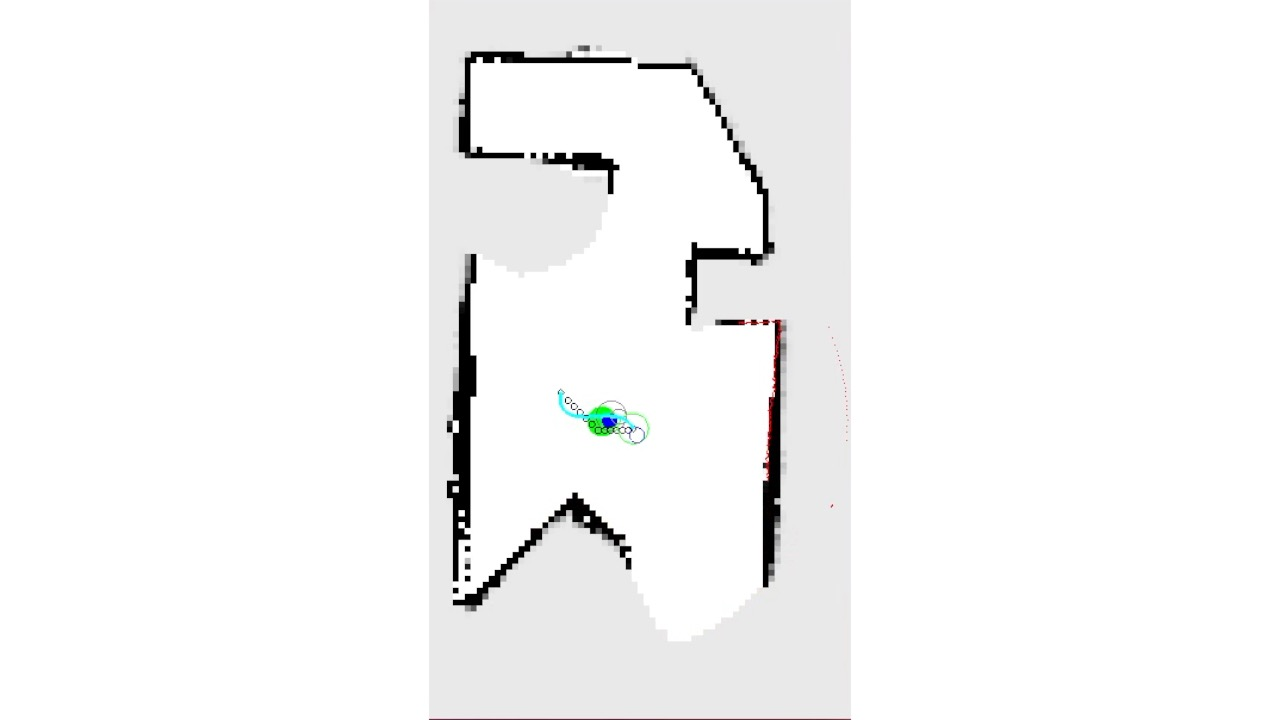
\includegraphics[trim={13cm 1cm 13cm 0}, clip, width=\textwidth]{t_3min.jpg}
        		\caption*{$t=3.0$min}
        		\label{fig:Experiment_ogm_t3}
    	\end{subfigure}    
	\begin{subfigure}[b]{0.19\textwidth}
        		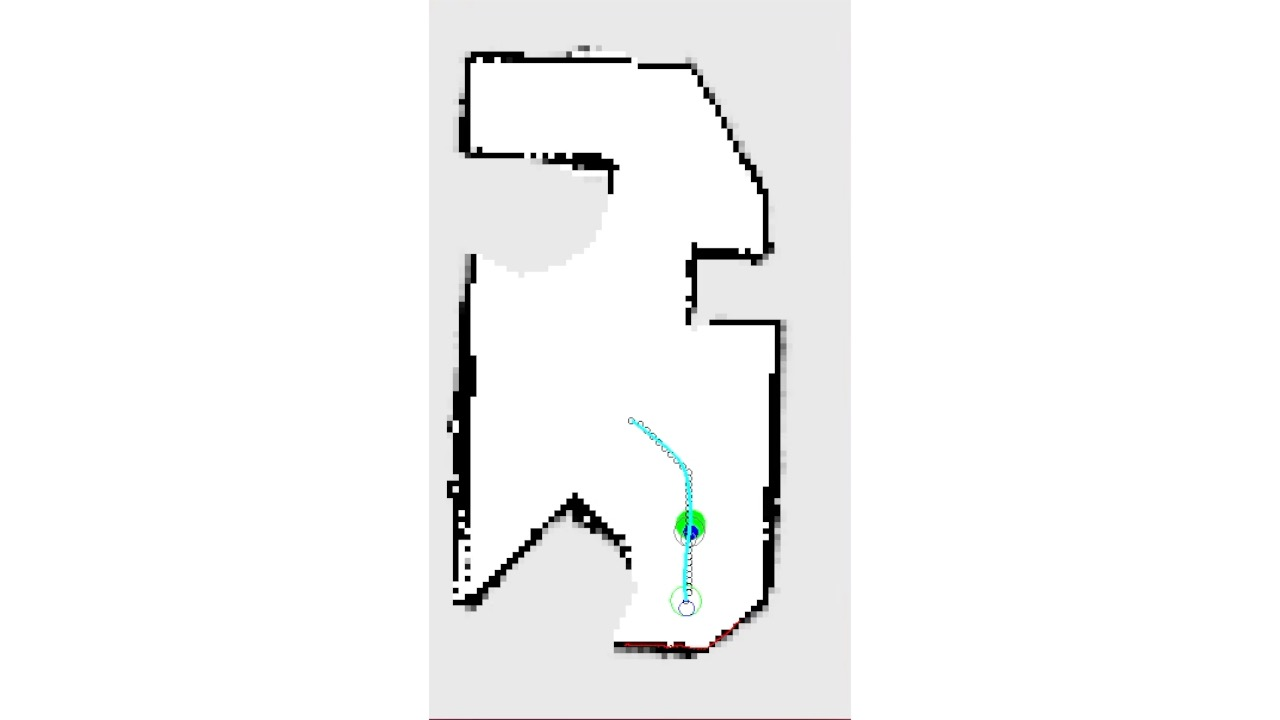
\includegraphics[trim={13cm 1cm 13cm 0}, clip, width=\textwidth]{t_3p5min.jpg}
        		\caption*{$t=3.5$min}
        		\label{fig:Experiment_ogm_t3p5}
    	\end{subfigure}
	\begin{subfigure}[b]{0.19\textwidth}
        		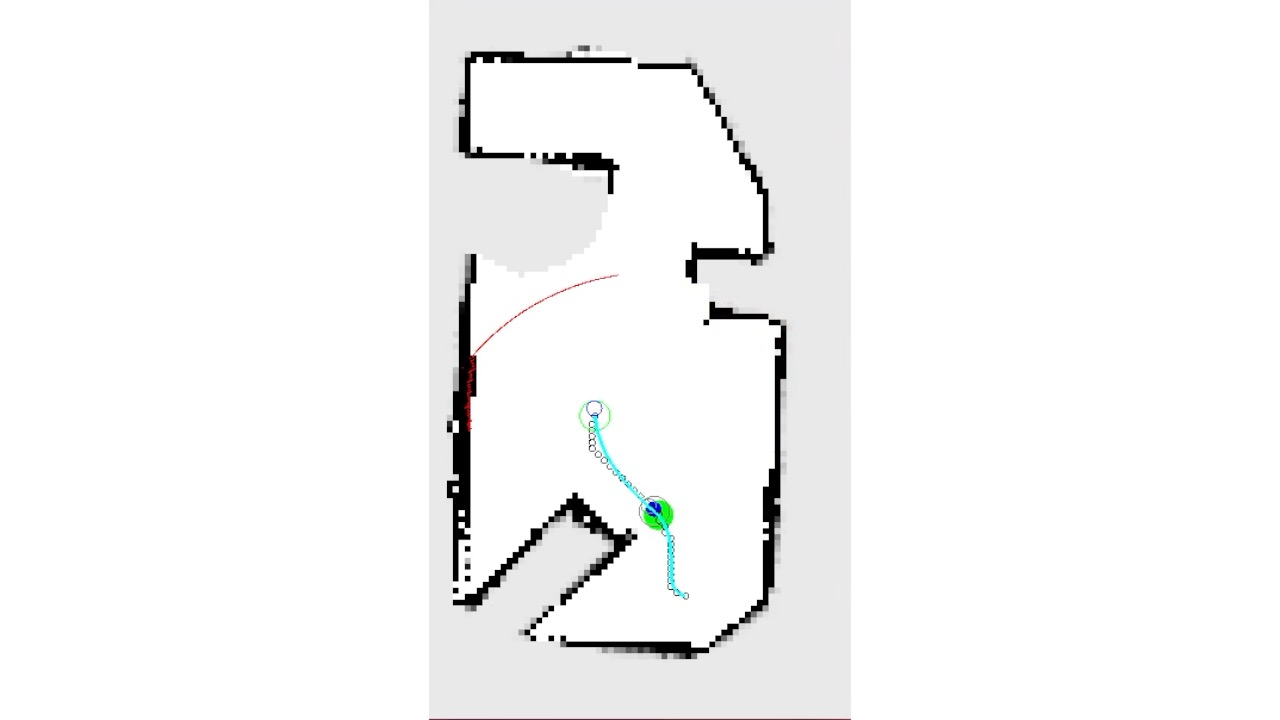
\includegraphics[trim={13cm 1cm 13cm 0}, clip, width=\textwidth]{t_4min.jpg}
        		\caption*{$t=4.0$min}
        		\label{fig:Experiment_ogm_t4}
    	\end{subfigure}
	\begin{subfigure}[b]{0.19\textwidth}
        		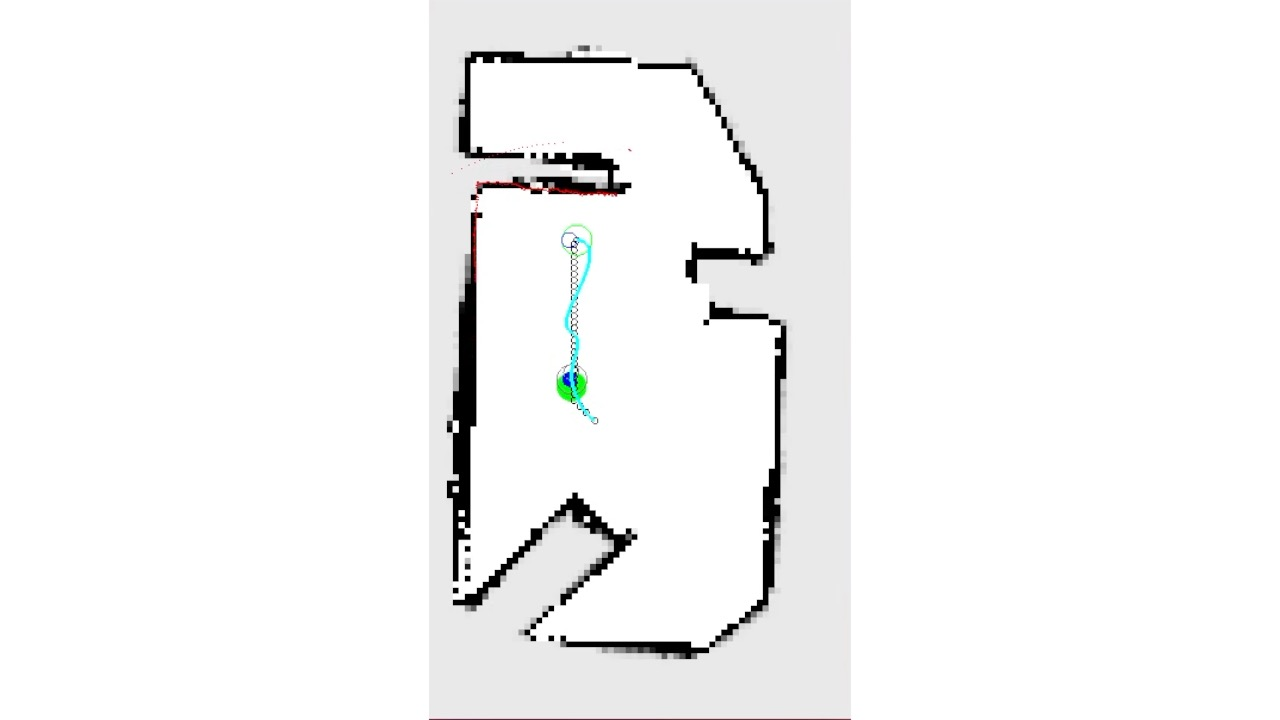
\includegraphics[trim={13cm 1cm 13cm 0}, clip, width=\textwidth]{t_4p5min.jpg}
        		\caption*{$t=4.5$min}
        		\label{fig:Experiment_ogm_t4p5}
    	\end{subfigure}
	}
\end{figure}

\end{frame}



\section*{}

\begin{frame}
\frametitle{}
%\center
\center{\bf \color{blue} Future Direction:\\Multi-Robot Autonomous Exploration}
\end{frame}

\subsection*{Future Direction: Multi-Robot Autonomous Exploration}

\begin{frame}
\frametitle{Proposed Topics}
\begin{itemize}
        	\item The ray-by-ray exact occupancy grid mapping approach in centralized probabilistic mapping
	\item Multiple robots choosing optimal motions considering each other
	\item Robots avoiding collisions with each other
	\item Coverage optimization of robots from different poses
\end{itemize}

\end{frame}

\begin{frame}
\frametitle{Proposed Future Steps}
\begin{itemize}
        	\item Mapping:
	\begin{itemize}
		\item Restructure algorithms for centralized map generation
		\item Communicate with multiple measurement sources
	\end{itemize}
	\item Exploration:
	\begin{itemize}
		\item Simplify enormous computation: bidding-based approach
		\item Temporary theoretical map building
		\item Collision avoidance between robots
	\end{itemize}
\end{itemize}

\end{frame}



\section*{}

\begin{frame}
\frametitle{}
%\center
\center{\bf \color{blue} Conclusions and Publications}
\end{frame}


\subsection*{Conclusions and Publications}

\begin{frame}
\frametitle{Conclusions}
\begin{itemize}
        	\item Proposed an occupancy grid mapping technique that uses the \emph{exact probabilistic solution}
	\item Computational cost is reduced \emph{substantially} for \emph{real-time implementation} using probabilisitic properties and exploiting mathematical patterns
	\item Exact mapping concepts are extended to map uncertainty to accomplish \emph{autonomous exploration}
	\item Proposing multiple vehicles can explore an uncertain environment using a \emph{bidding}-based approach
\end{itemize}
\end{frame}

\begin{frame}
\frametitle{Publications}
{\tiny 
\begin{itemize}
	\item E. Kaufman, K. Takami, T. Lee, and Z. Ai, ``Autonomous Exploration with Exact Inverse Sensor Models,'' \textit{Journal of Intelligent }\&\textit{ Robotic Systems}, 2016, submitted.
	\item E. Kaufman, T. Lee, and Z. Ai, ``Autonomous Exploration by Expected Information Gain from Probabilistic Occupancy Grid Mapping,'' \textit{IEEE International Conference on Simulation, Modeling, and Programming for Autonomous Robots}, San Francisco, December 2016, accepted.
	\item E. Kaufman, T. Lee, Z. Ai, and I. S. Moskowitz, ``Bayesian Occupancy Grid Mapping via an Exact Inverse Sensor Model,'' \textit{Proceedings of the American Control Conference}, Boston, July 2016, pp. 5709-5715.
	\item E. Kaufman, T. A. Lovell, and T. Lee, ``Nonlinear Observability Measure for Relative Orbit Determination with Angles-Only Measurements,'' \textit{The Journal of the Astronautical Sciences}, 63(1): pp. 60-80, 2016, doi: 10.1007/s40295-015-0082-9.
	\item E. Kaufman, T. A. Lovell, and T. Lee, ``Minimum Uncertainty JPDA Filters and Coalescence Avoidance for Multiple Object Tracking,'' \textit{The Journal of the Astronautical Sciences}, 63(4): pp. 308-334, 2016, doi: 10.1007/s40295-016-0092-2.
	\item T. Wu, E. Kaufman, and T. Lee, ``Globally Asymptotically Stable Attitude Observer on SO(3),'' \textit{Proceedings of the 54th IEEE Conference on Decision and Control}, pp. 2164-2168, Osaka, Japan, December 2015.
	\item E. Kaufman, T. A. Lovell, and T. Lee, ``Nonlinear Observability Measure for Relative Orbit Determination with Angles-Only Measurements,'' \textit{Proceedings of the 25th AAS/AIAA Space Flight Mechanics Meeting}, Williamsburg, VA, Jan. 2015, AAS 15-451.
	\item E. Kaufman, T. A. Lovell, and T. Lee, ``Minimum Uncertainty JPDA Filter and Coalescence Avoidance Performance Evaluations,'' \textit{Proceedings of the 25th AAS/AIAA Space Flight Mechanics Meeting, Williamsburg}, VA, Jan. 2015, AAS 15-432.
	\item E. Kaufman, K. Caldwell, D. Lee, and T. Lee, ``Design and Development of a Free-Floating Hexrotor UAV for 6-DOF Maneuvers,'' \textit{Proceedings of the IEEE Aerospace Conference}, Mar. 2014, ASC 14-2527.
	\item E. Kaufman, T. A. Lovell, and T. Lee, ``Optimal Joint Probabilistic Data Association Filter Avoiding Coalescence in Close Proximity,'' \textit{Proceedings of the European Control Conference}, pp. 2709-2714, June 2014.
	\vspace*{0.5cm}
\end{itemize}
}
\end{frame}




\end{document}

